\chapter{Appendix A}

\section{Additional Apparatus Pictures} \label{sec:additional_apparatus}

\begin{figure}[htpb]
    \centering
    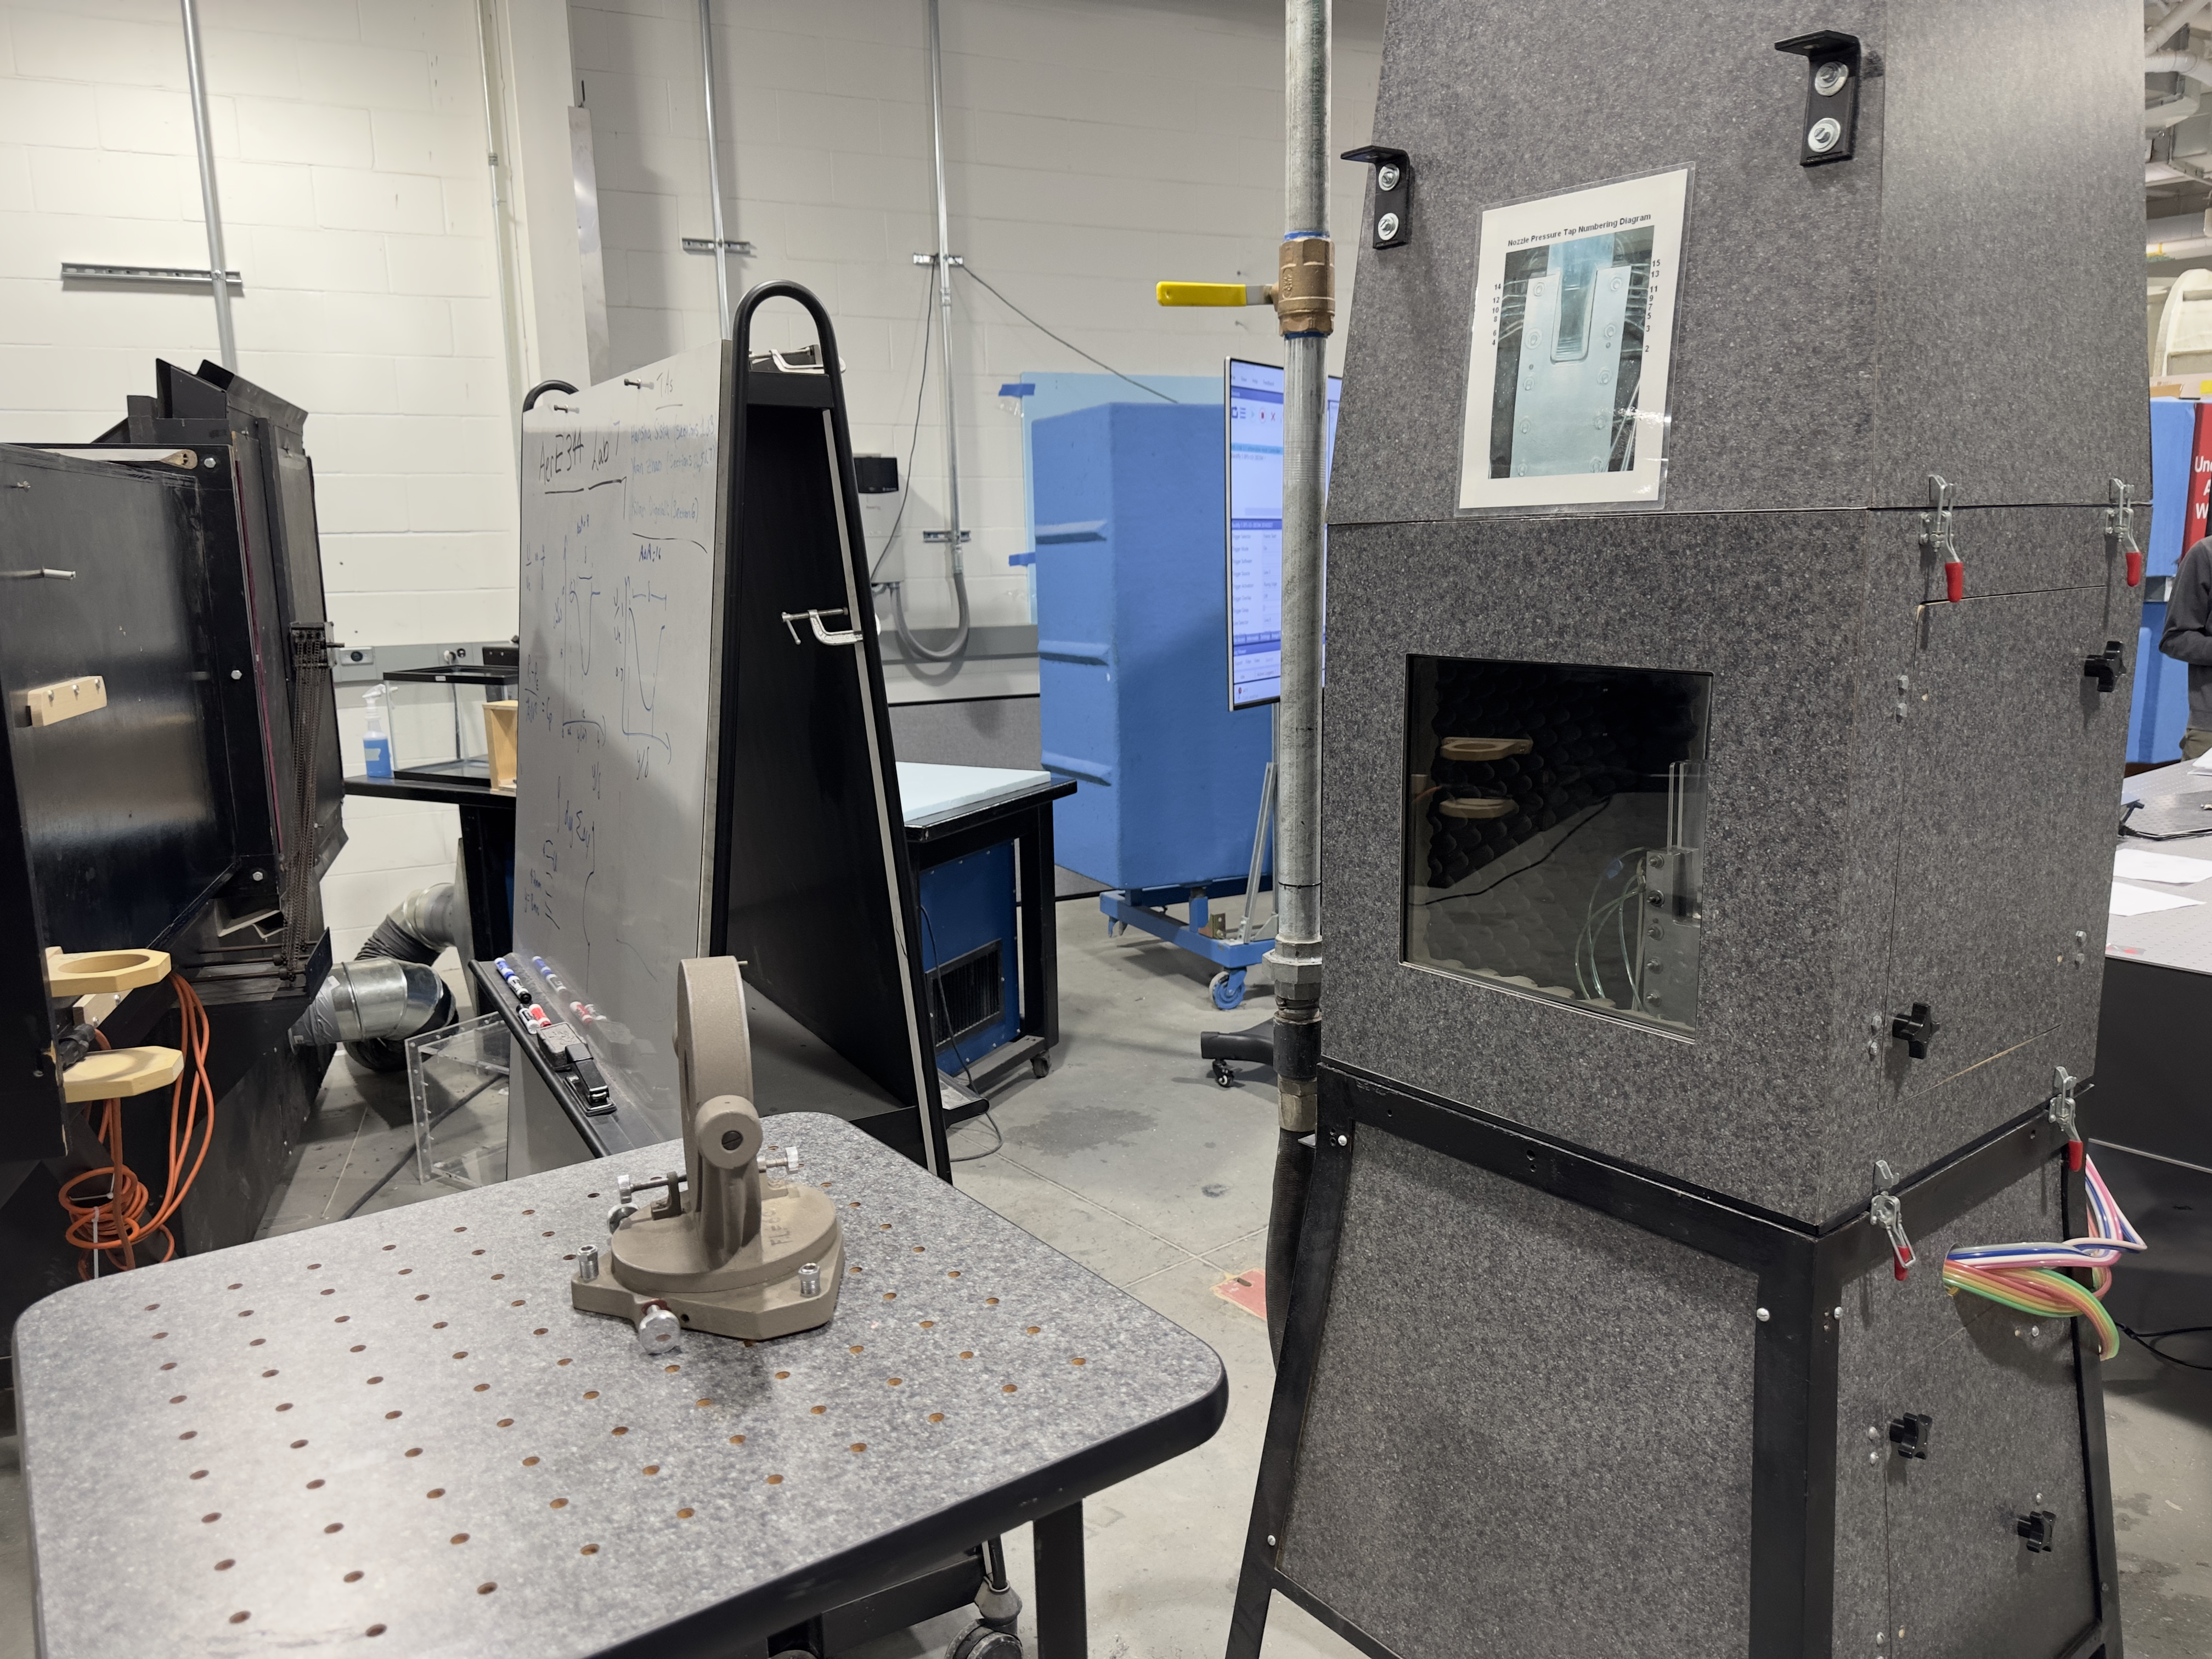
\includegraphics[width=0.75\linewidth]{Figures/back_of_supersonic_wind_tunnel.jpeg}
    \caption[Supersonic Wind tunnel apparatus]{Supersonic Wind tunnel apparatus}
    \label{fig: SuperSonicWindTunnel}
\end{figure}

\begin{figure}[htpb]
    \centering
    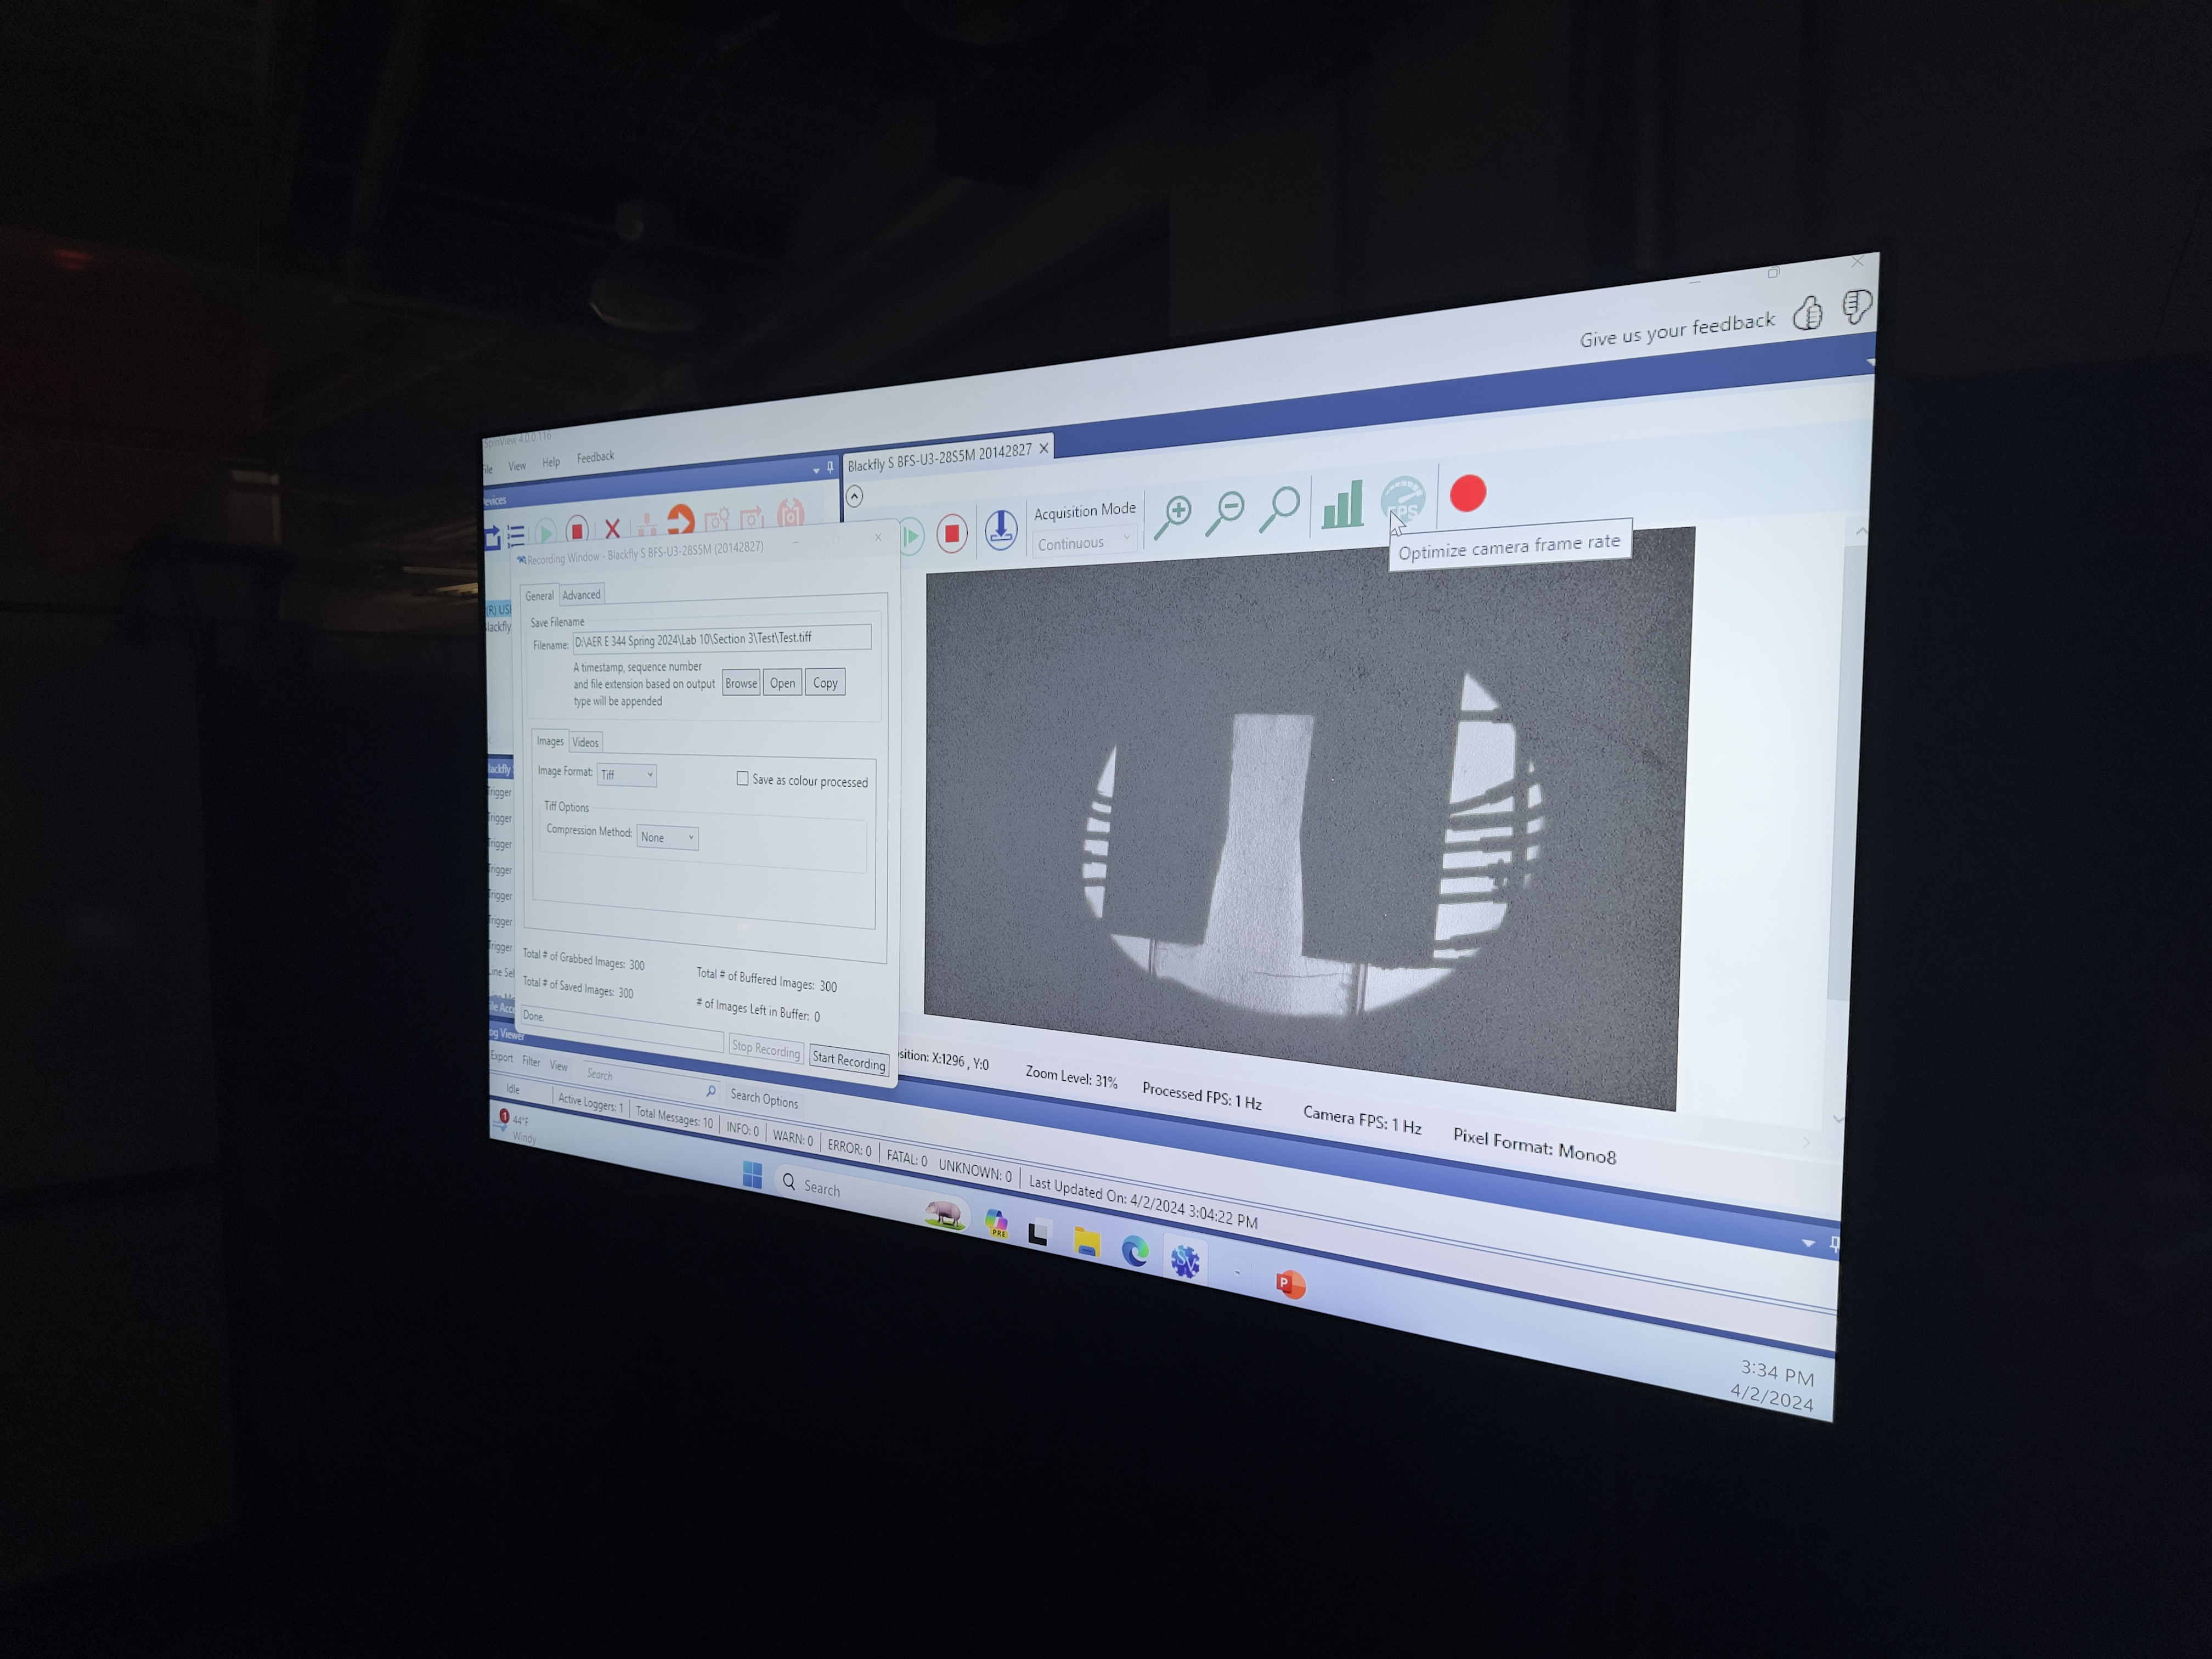
\includegraphics[width=0.75\linewidth]{Figures/camera_capture_settings.jpeg}
    \caption[Camera Capture Settings]{Camera Capture Settings}
    \label{fig: CameraCaptureSettings}
\end{figure}

\begin{figure}[htpb]
    \centering
    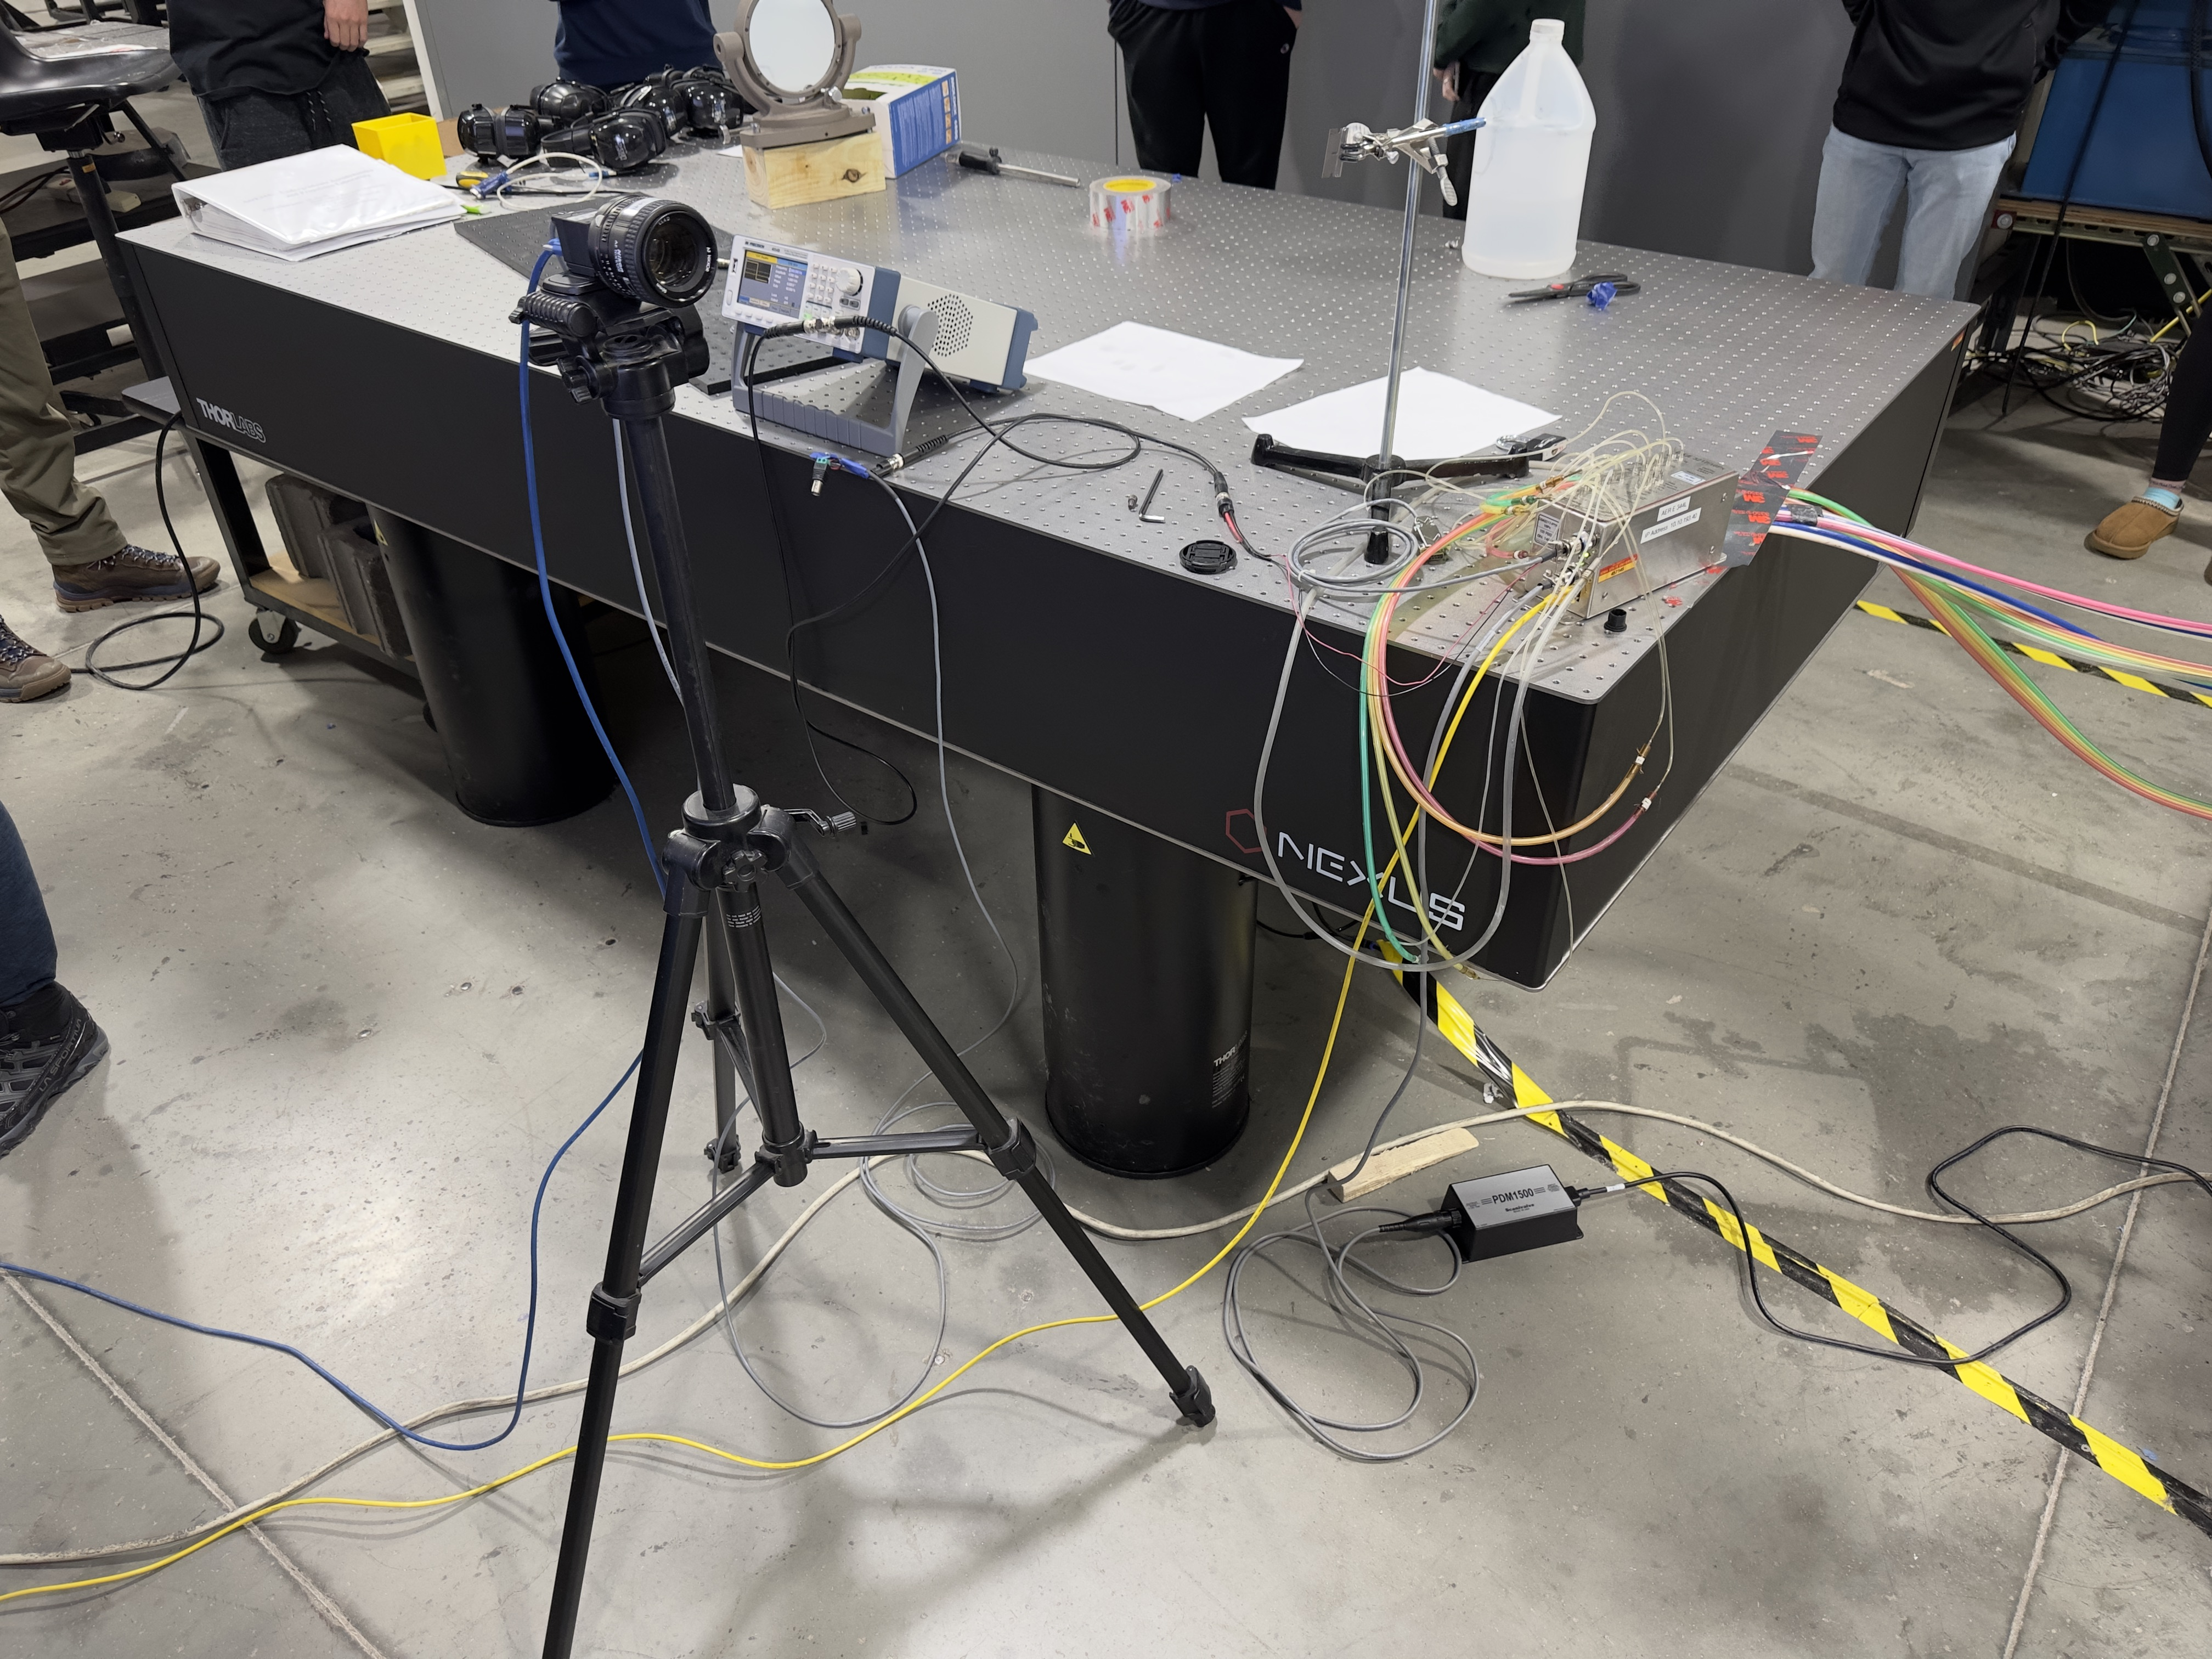
\includegraphics[width=0.75\linewidth]{Figures/camera.jpeg}
    \caption[Camera]{Camera}
    \label{fig: Camera}
\end{figure}

\begin{figure}[htpb]
    \centering
    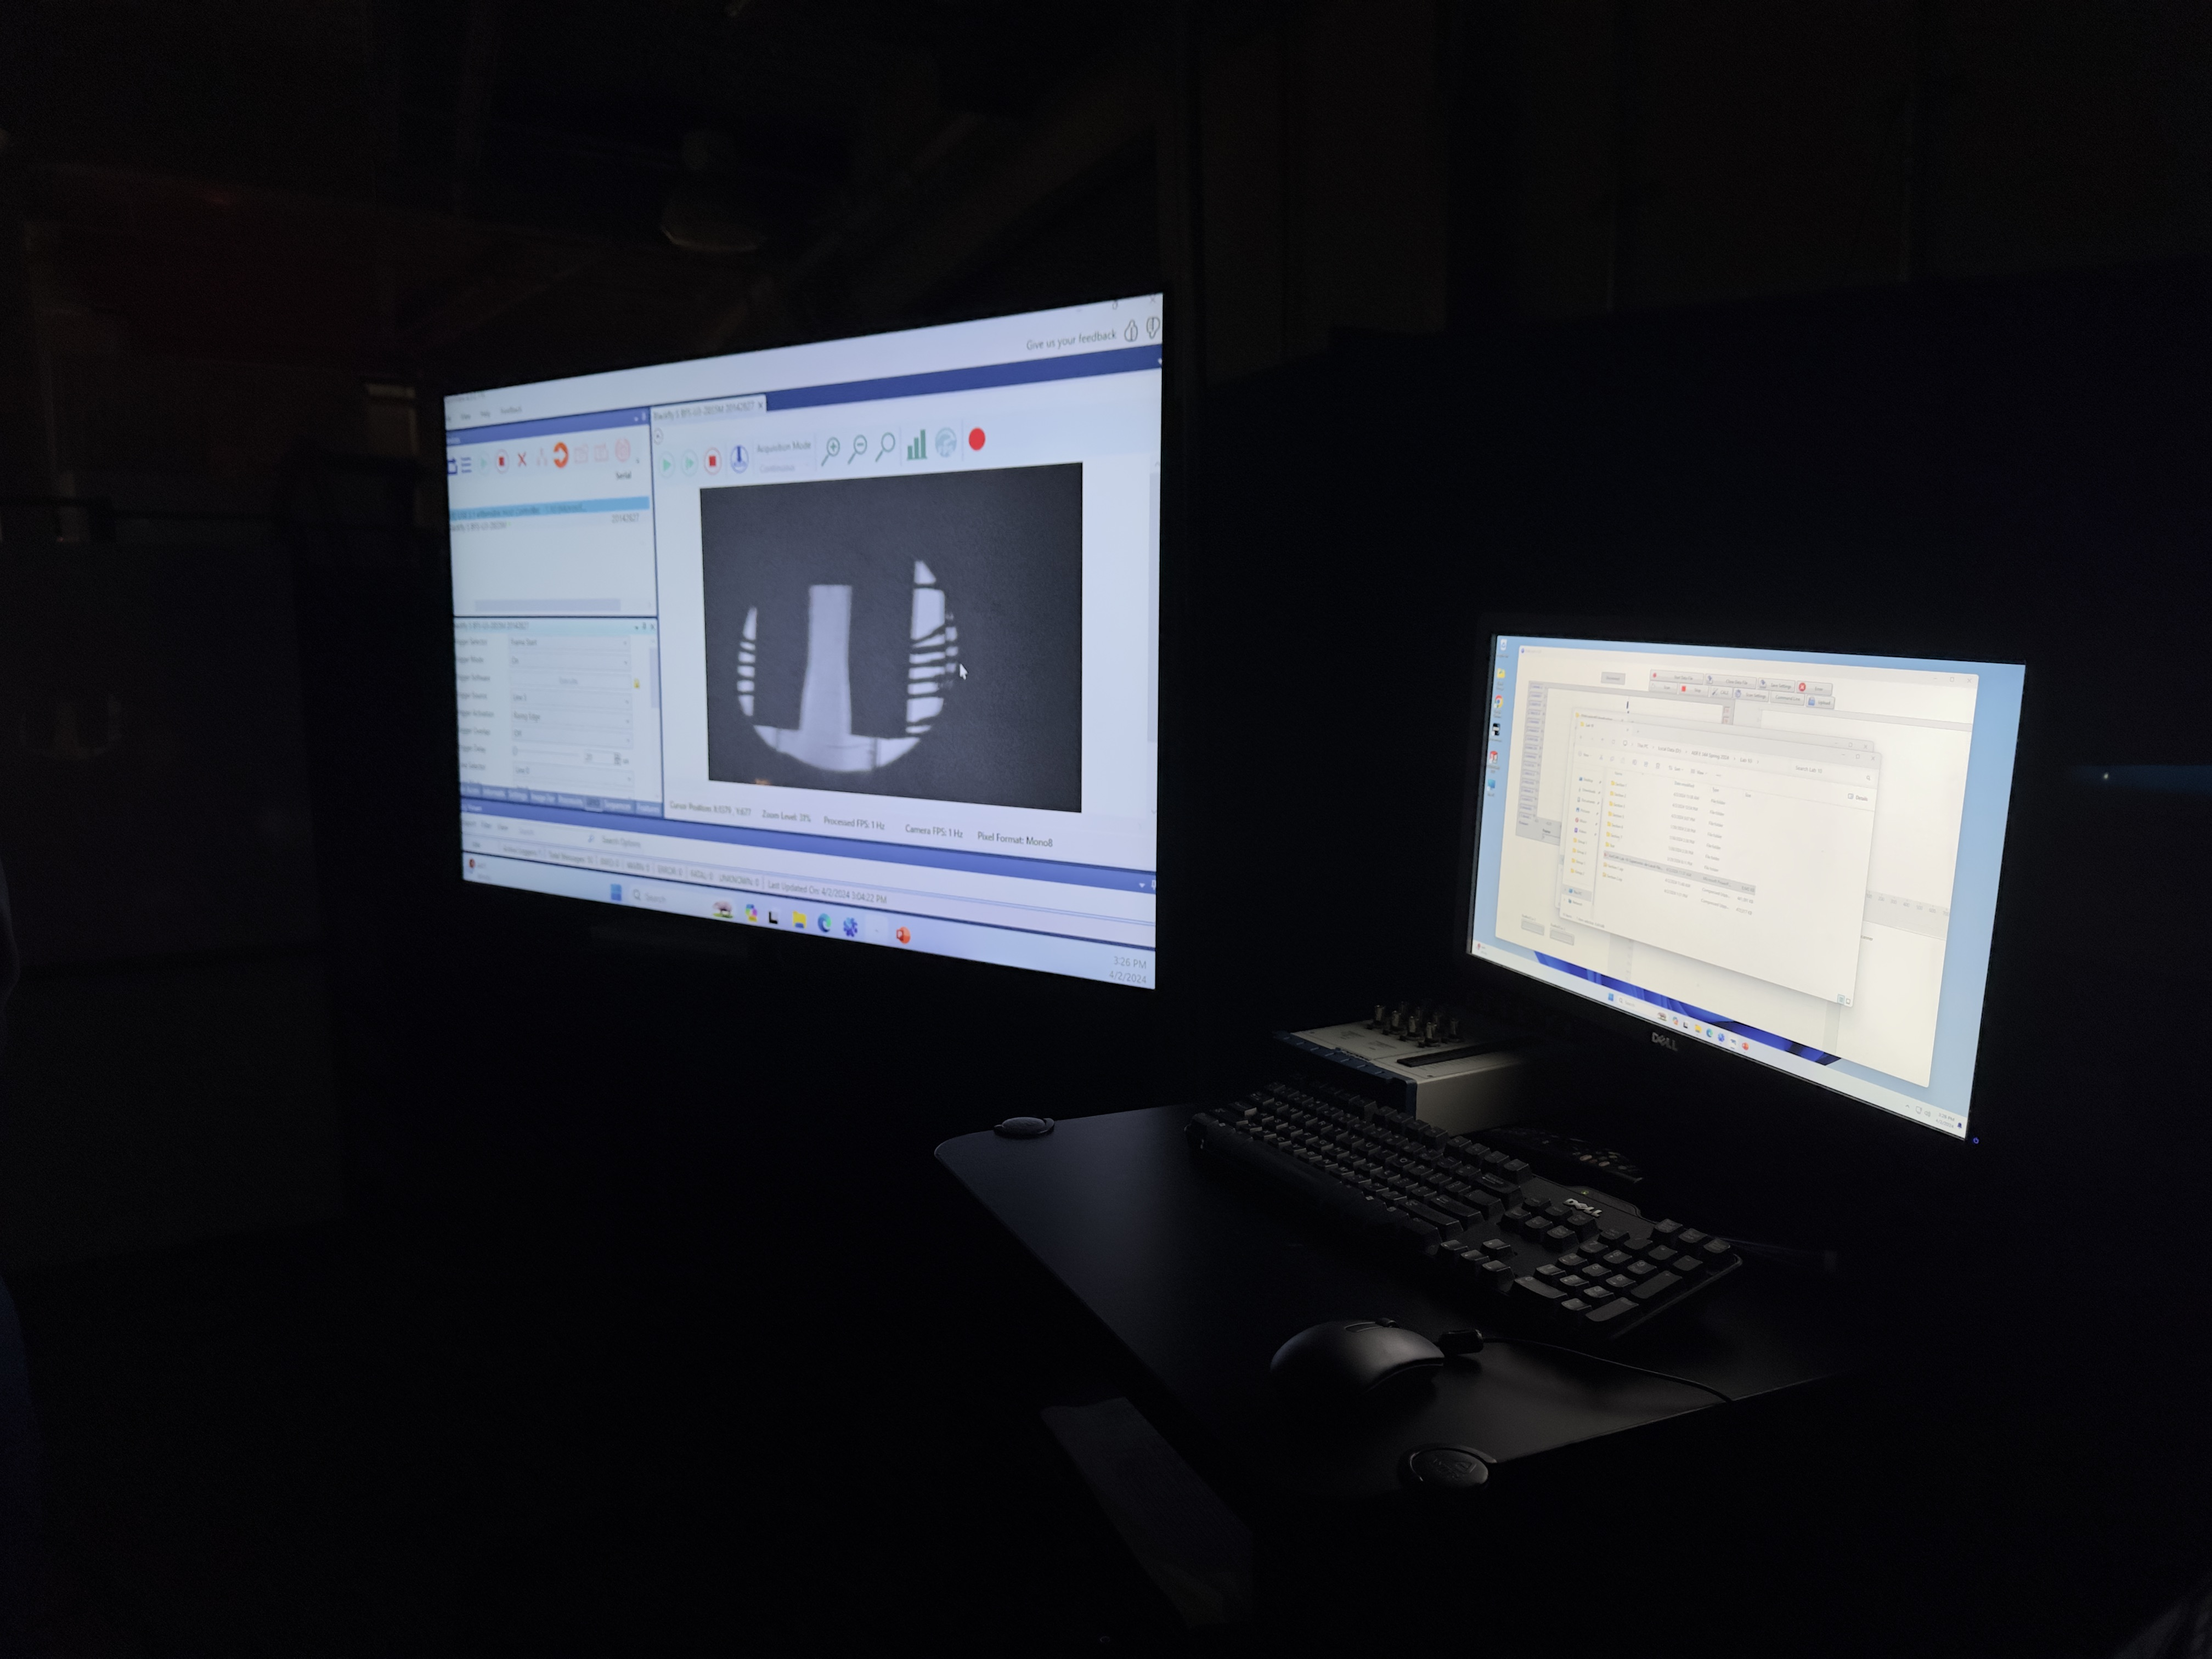
\includegraphics[width=0.75\linewidth]{Figures/data_acquisition_software.jpeg}
    \caption[Data Acquisition Software]{Data Acquisition Software}
    \label{fig: DataAcquisition}
\end{figure}

\begin{figure}[htpb]
    \centering
    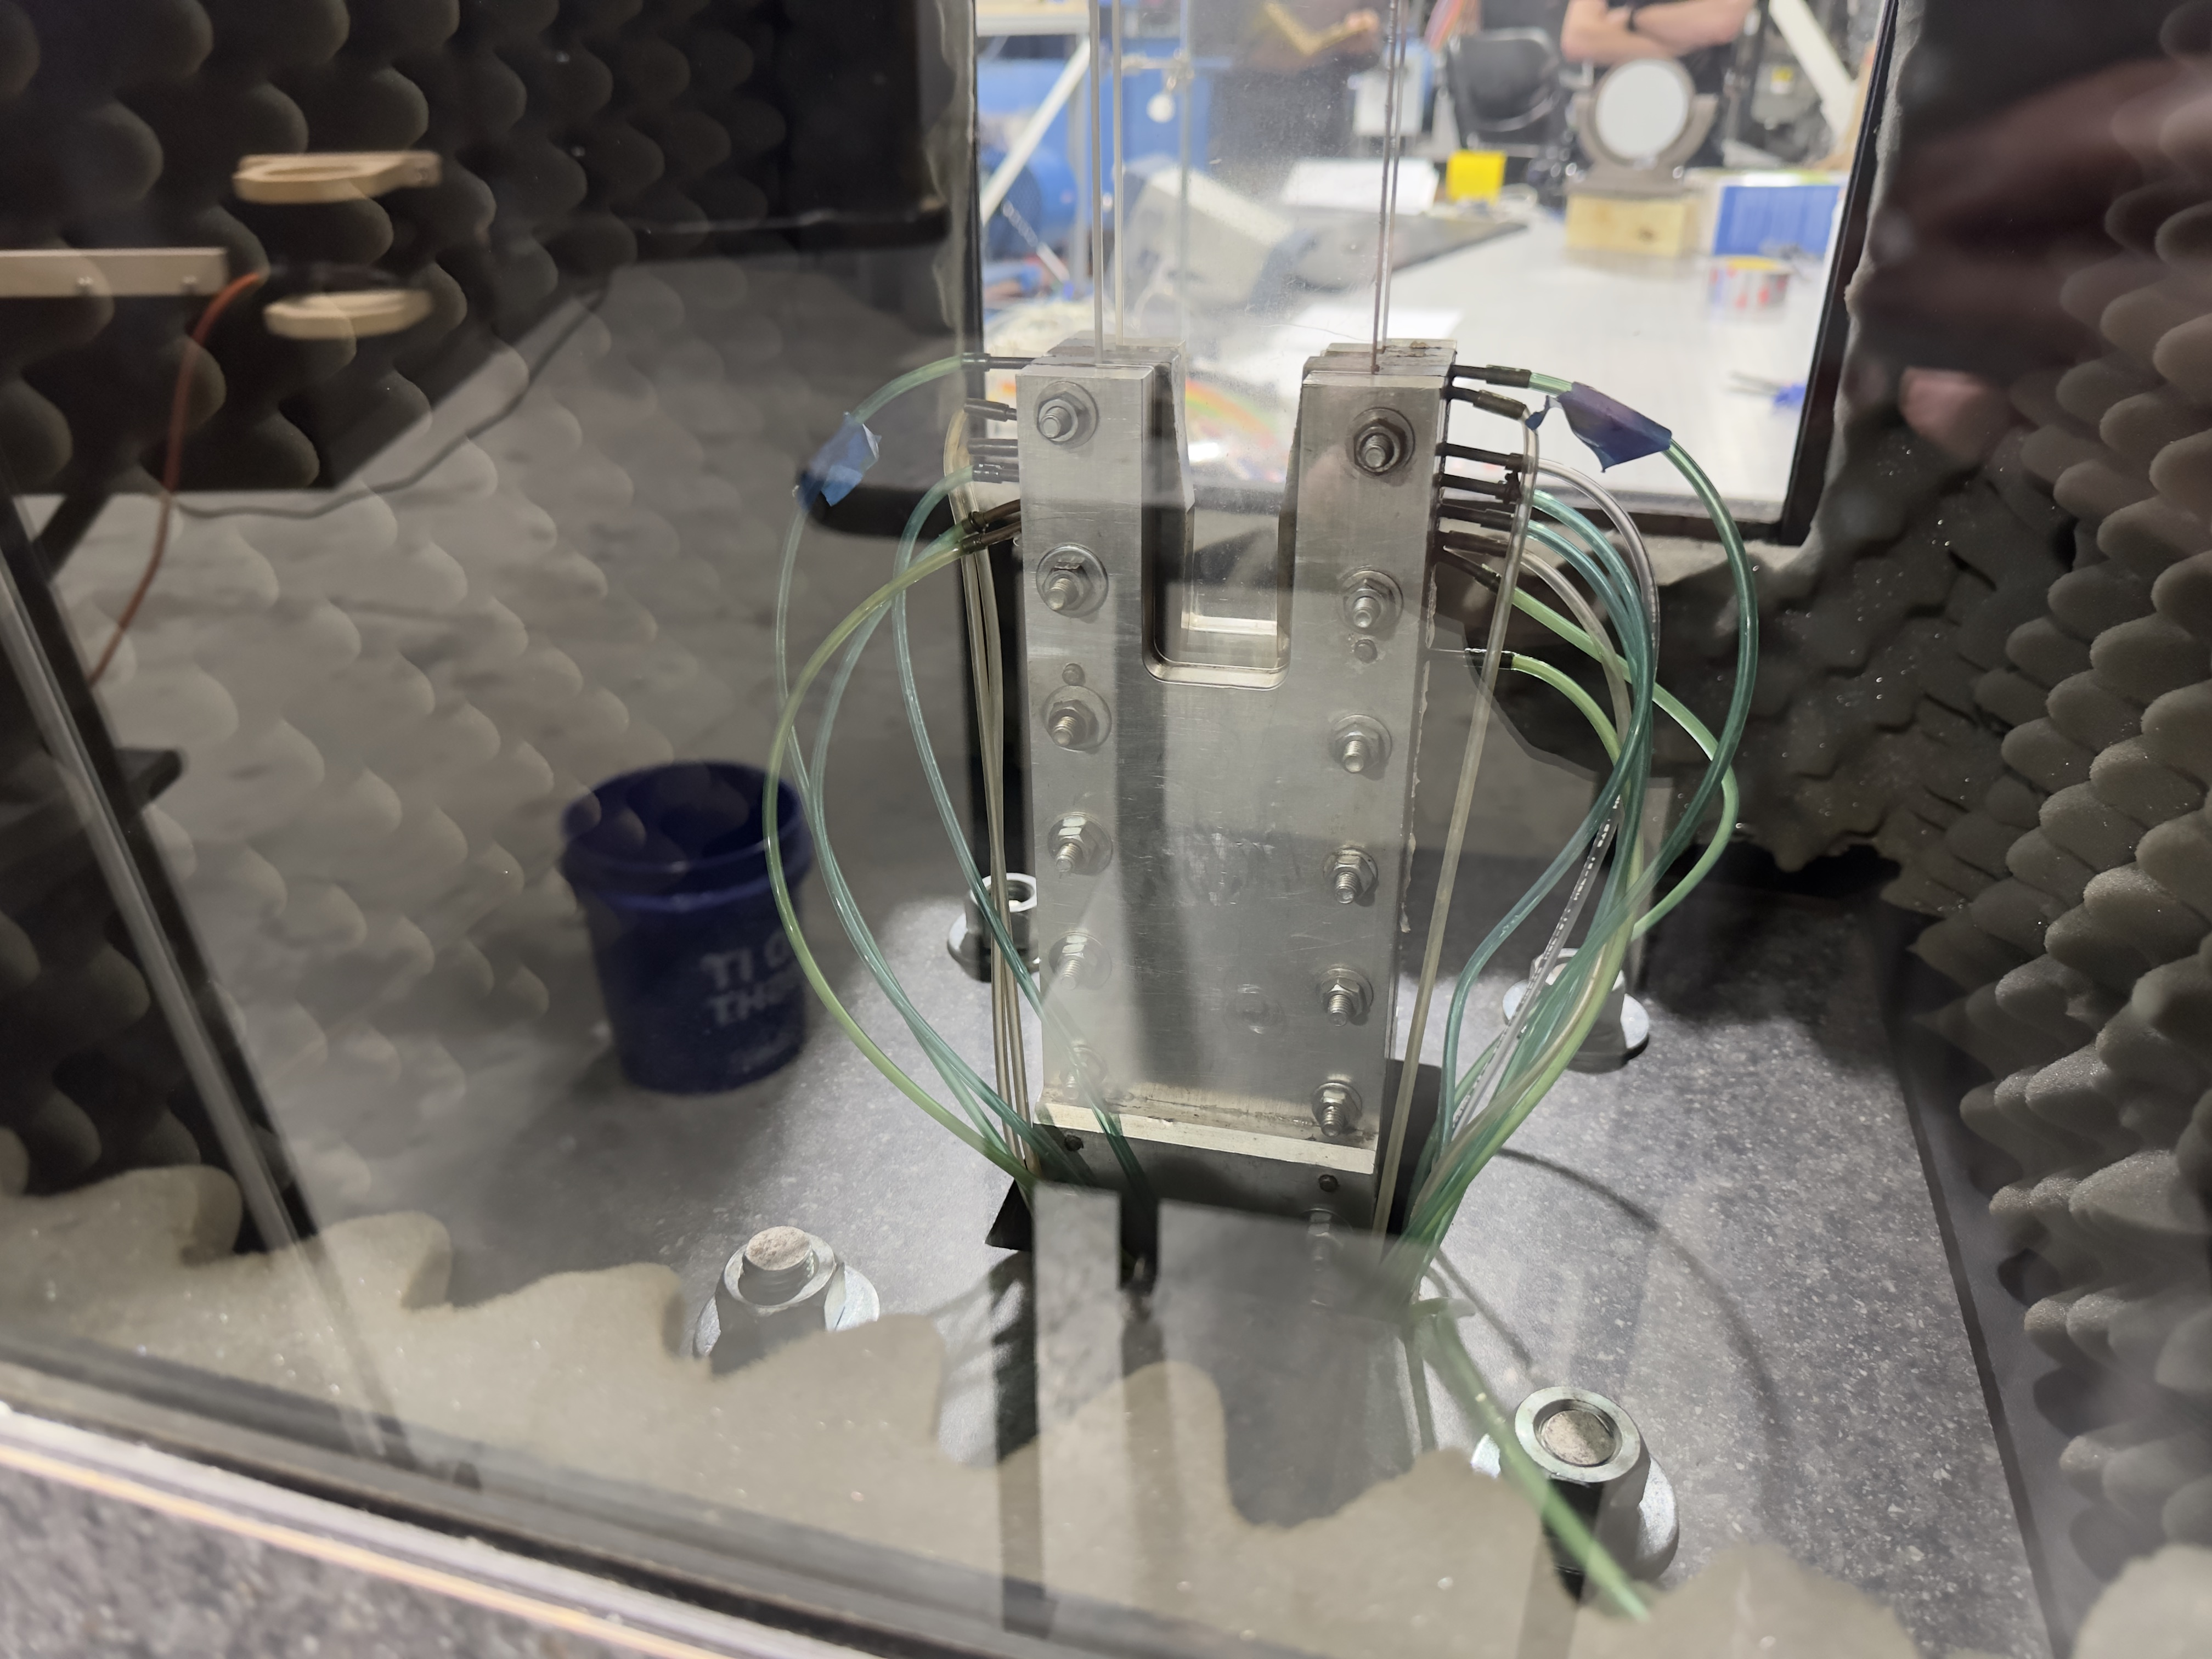
\includegraphics[width=0.75\linewidth]{Figures/de_laval_nozzle.jpeg}
    \caption[de Laval Nozzle]{de Laval Nozzle}
    \label{fig: deLavalNozzle}
\end{figure}

\begin{figure}[htpb]
    \centering
    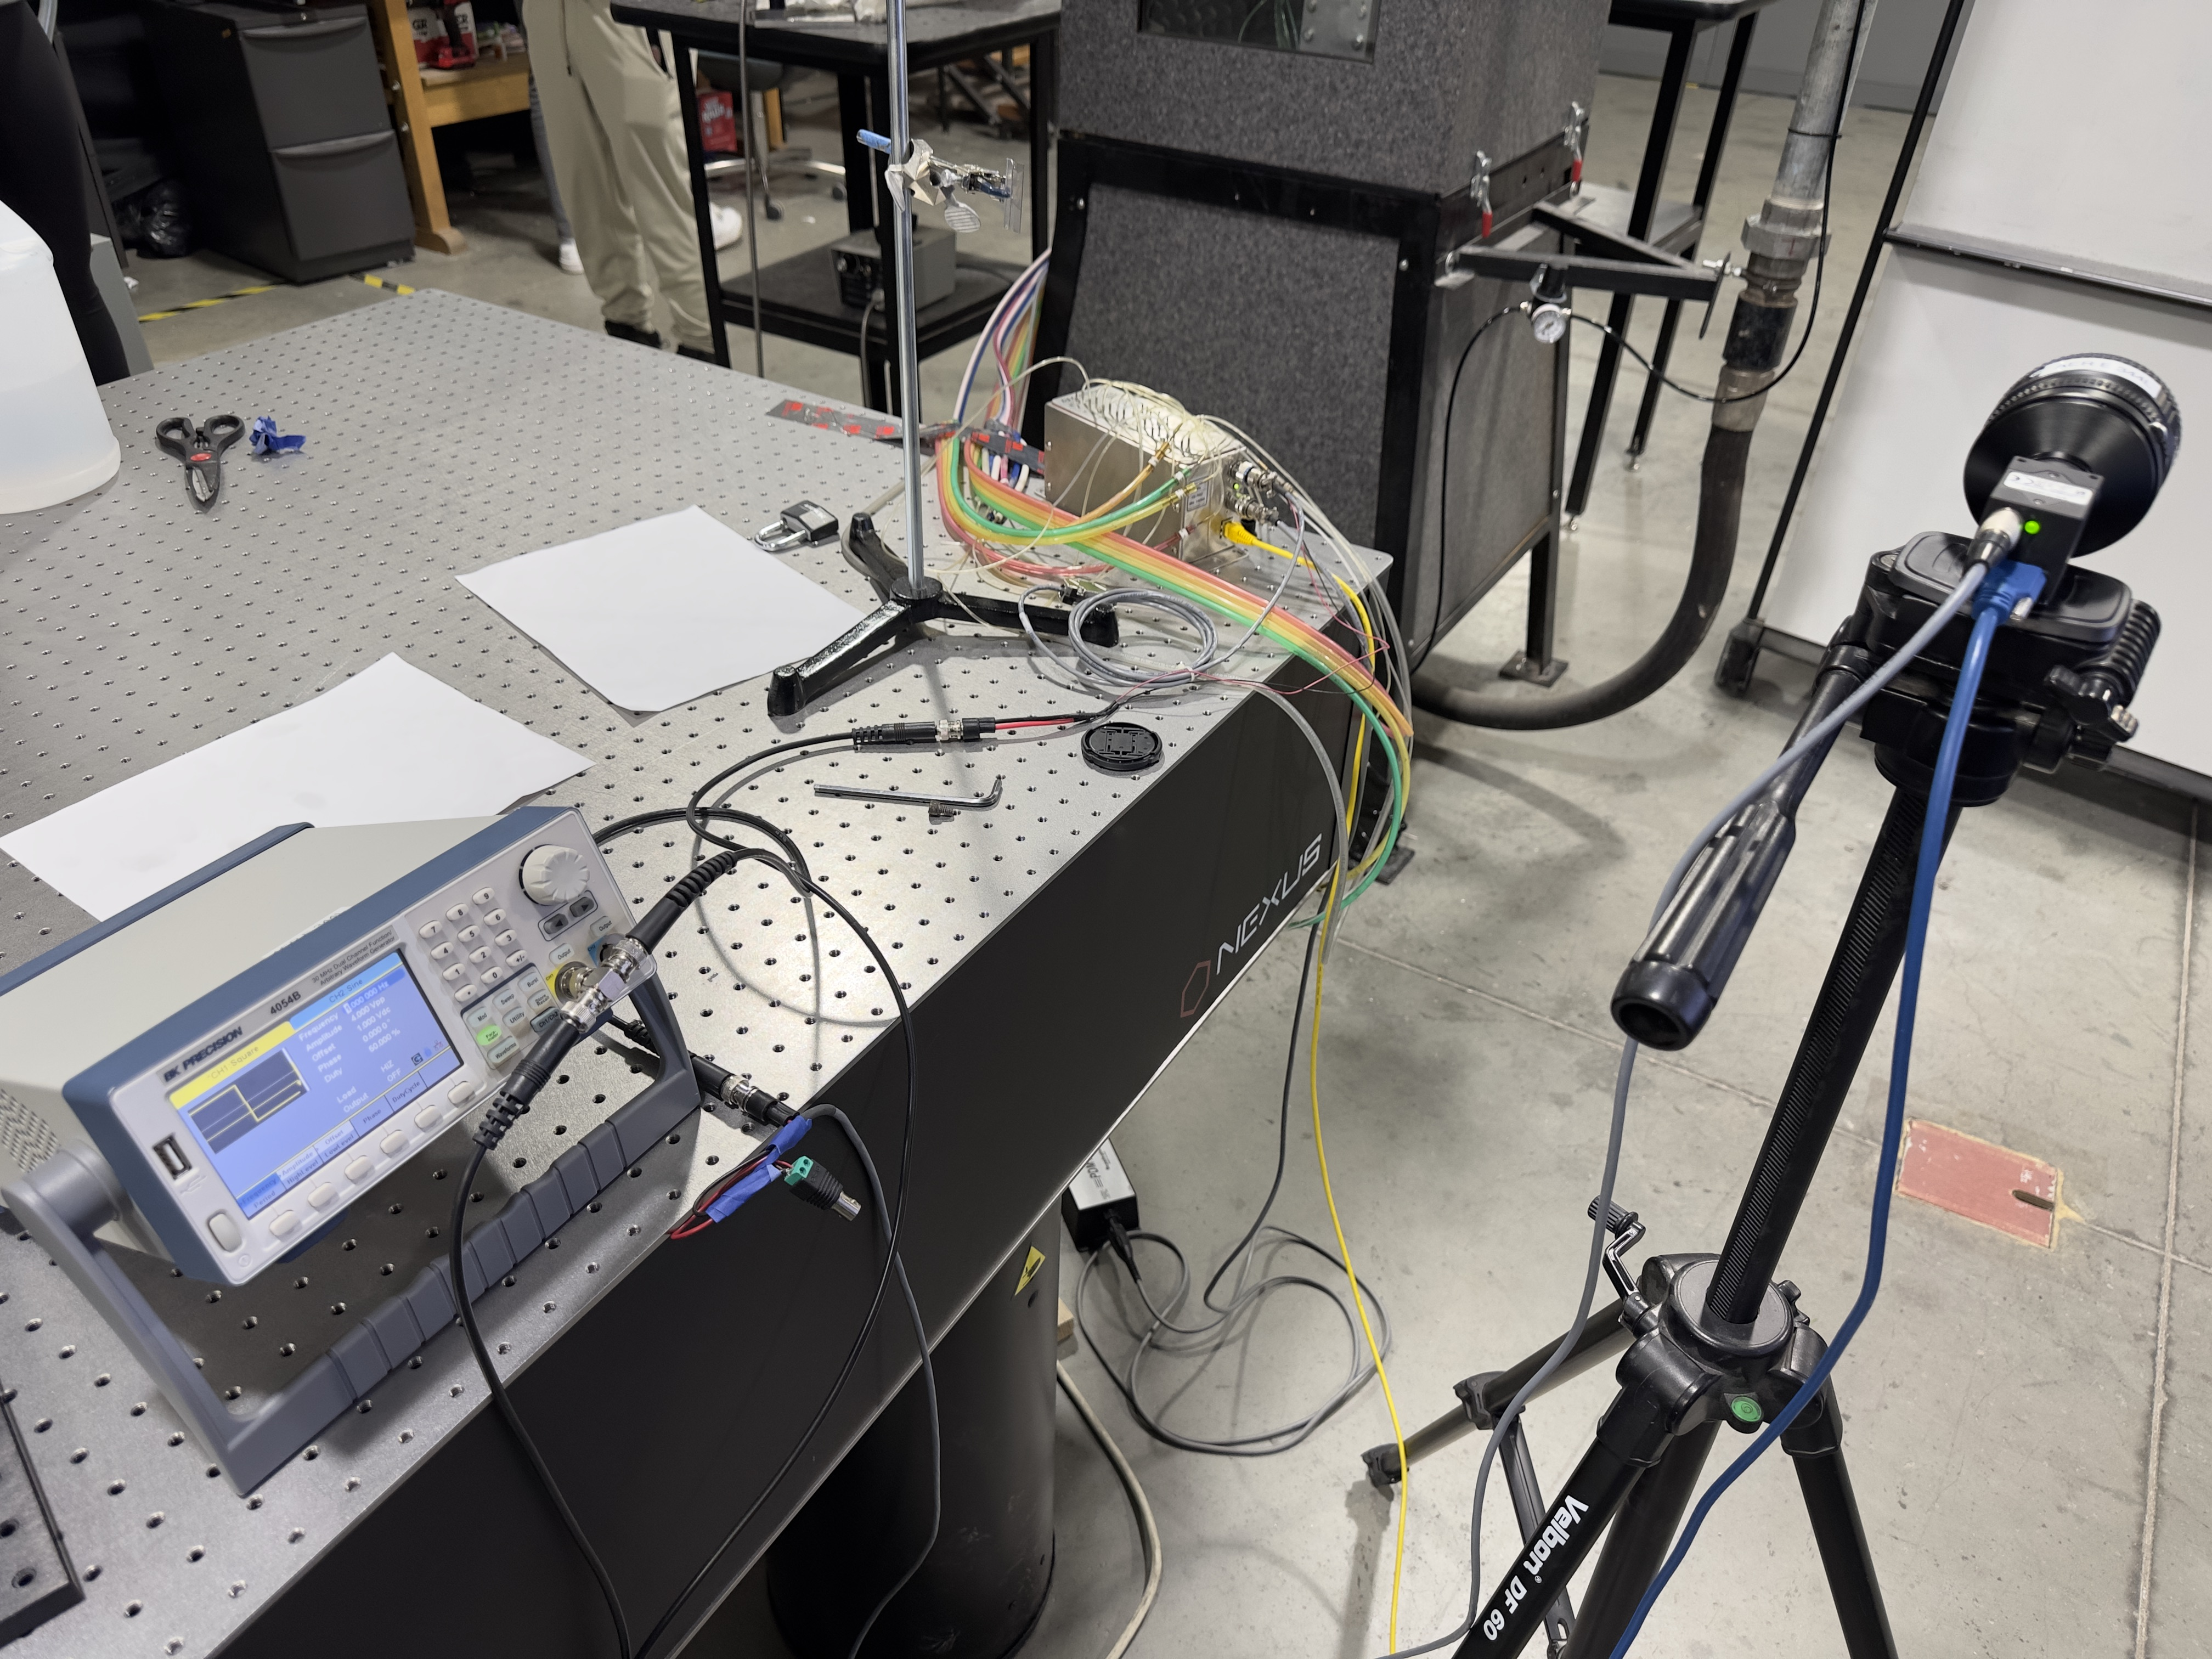
\includegraphics[width=0.75\linewidth]{Figures/delay_generator_and_schlieren.jpeg}
    \caption[Delay Generator and Schlieren Settup]{Delay Generator and Schlieren Setup}
    \label{fig: delayGeneratoandSchlieren}
\end{figure}

\begin{figure}[htpb]
    \centering
    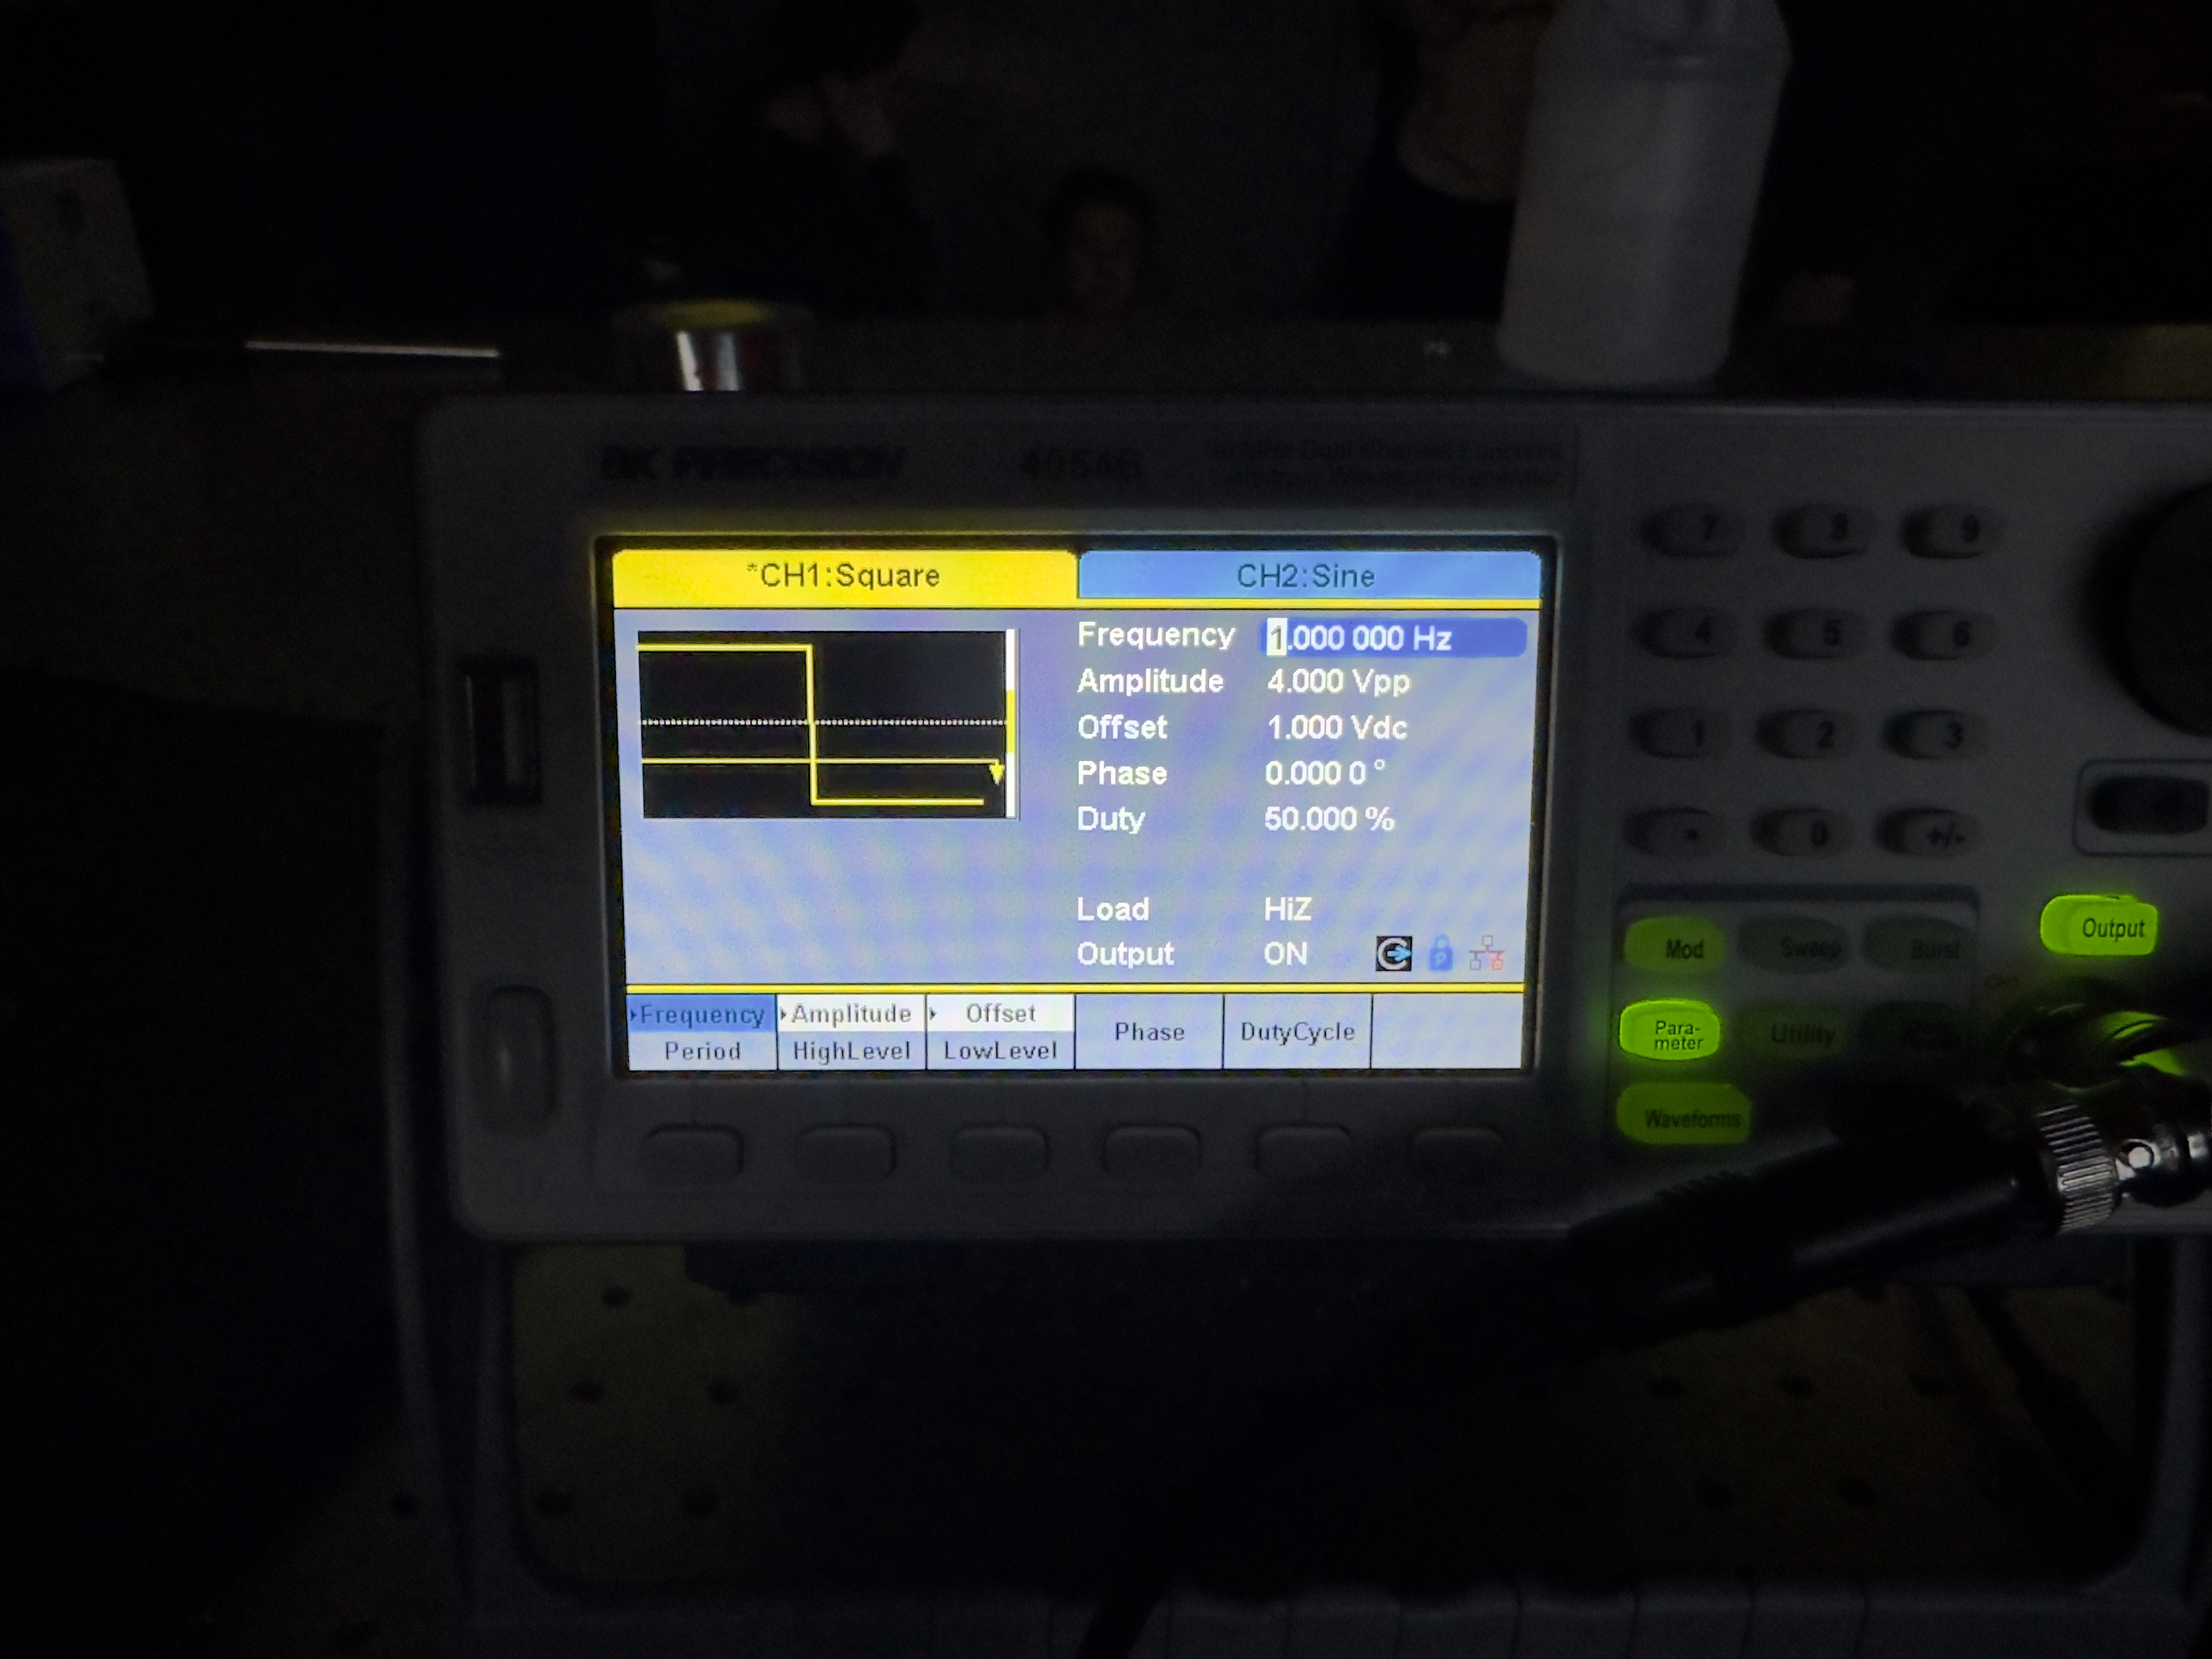
\includegraphics[width=0.75\linewidth]{Figures/delay_generator_settings.jpeg}
    \caption[Delay Generator Settings]{Delay Generator Settings}
    \label{fig: delayGeneratorsettings}
\end{figure}

\begin{figure}[htpb]
    \centering
    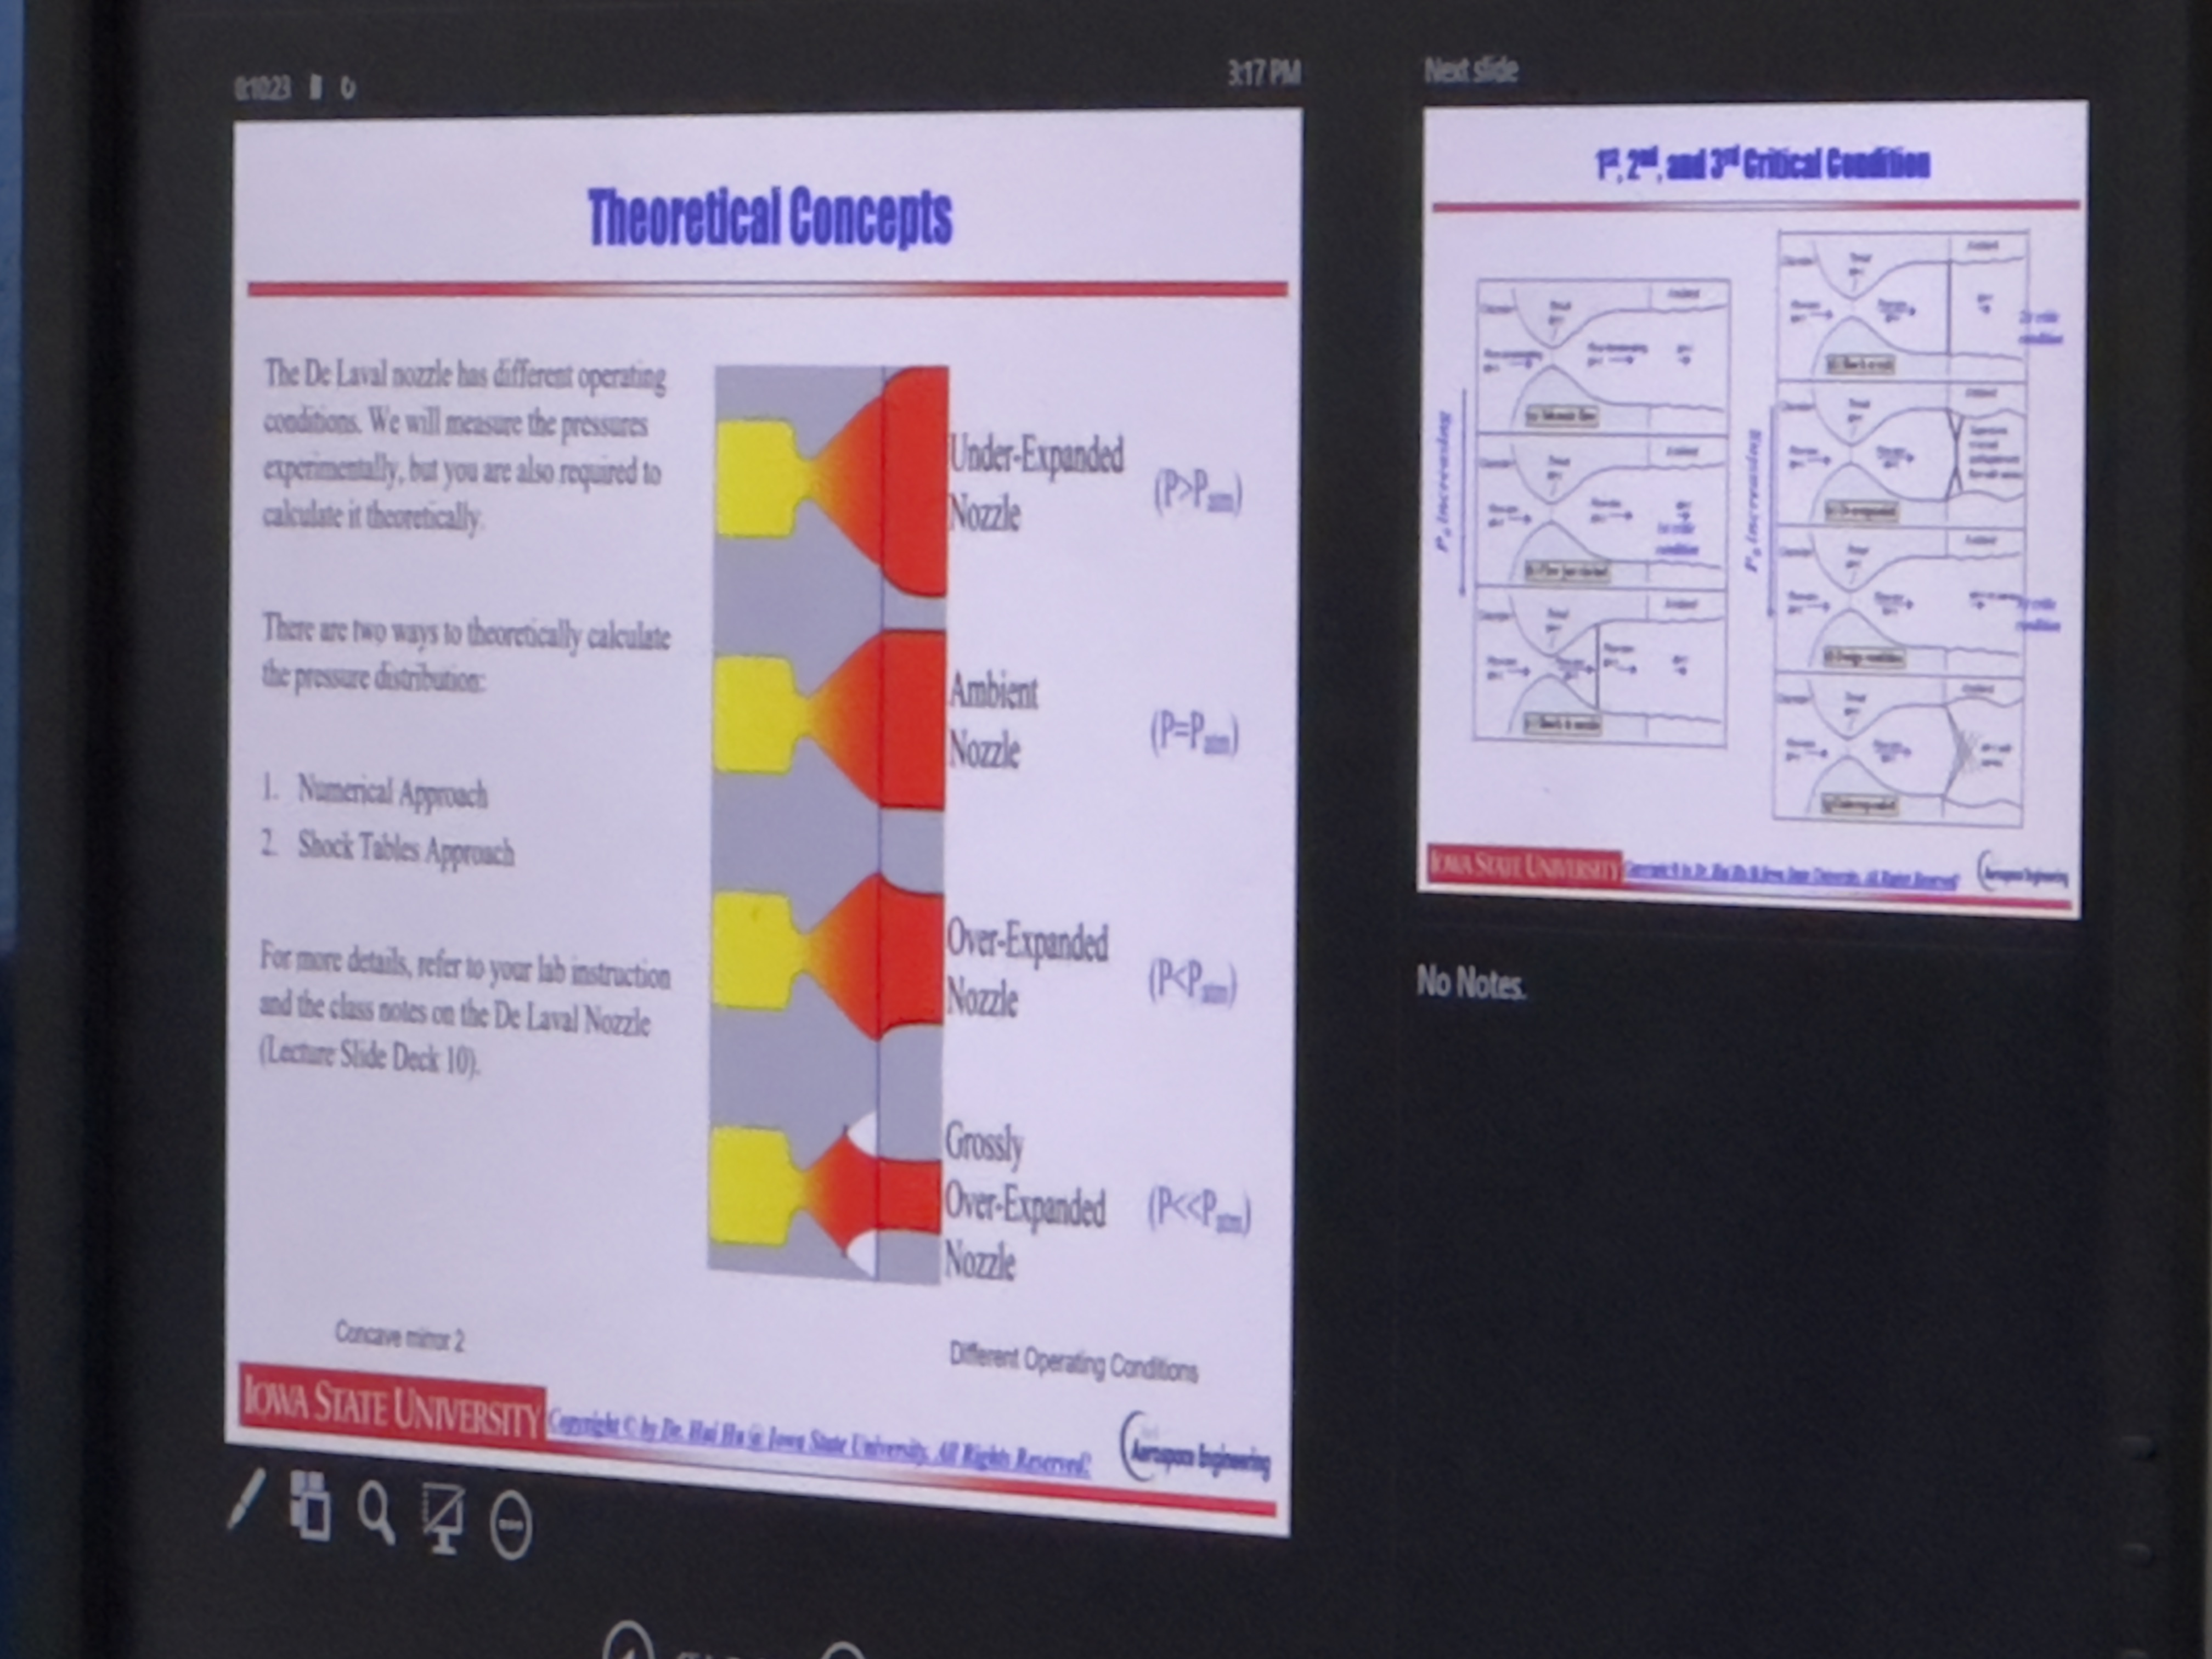
\includegraphics[width=0.75\linewidth]{Figures/different_flows.jpeg}
    \caption[Different Flows]{Diffrent Flows}
    \label{fig: DiffrentFlows}
\end{figure}

\begin{figure}[htpb]
    \centering
    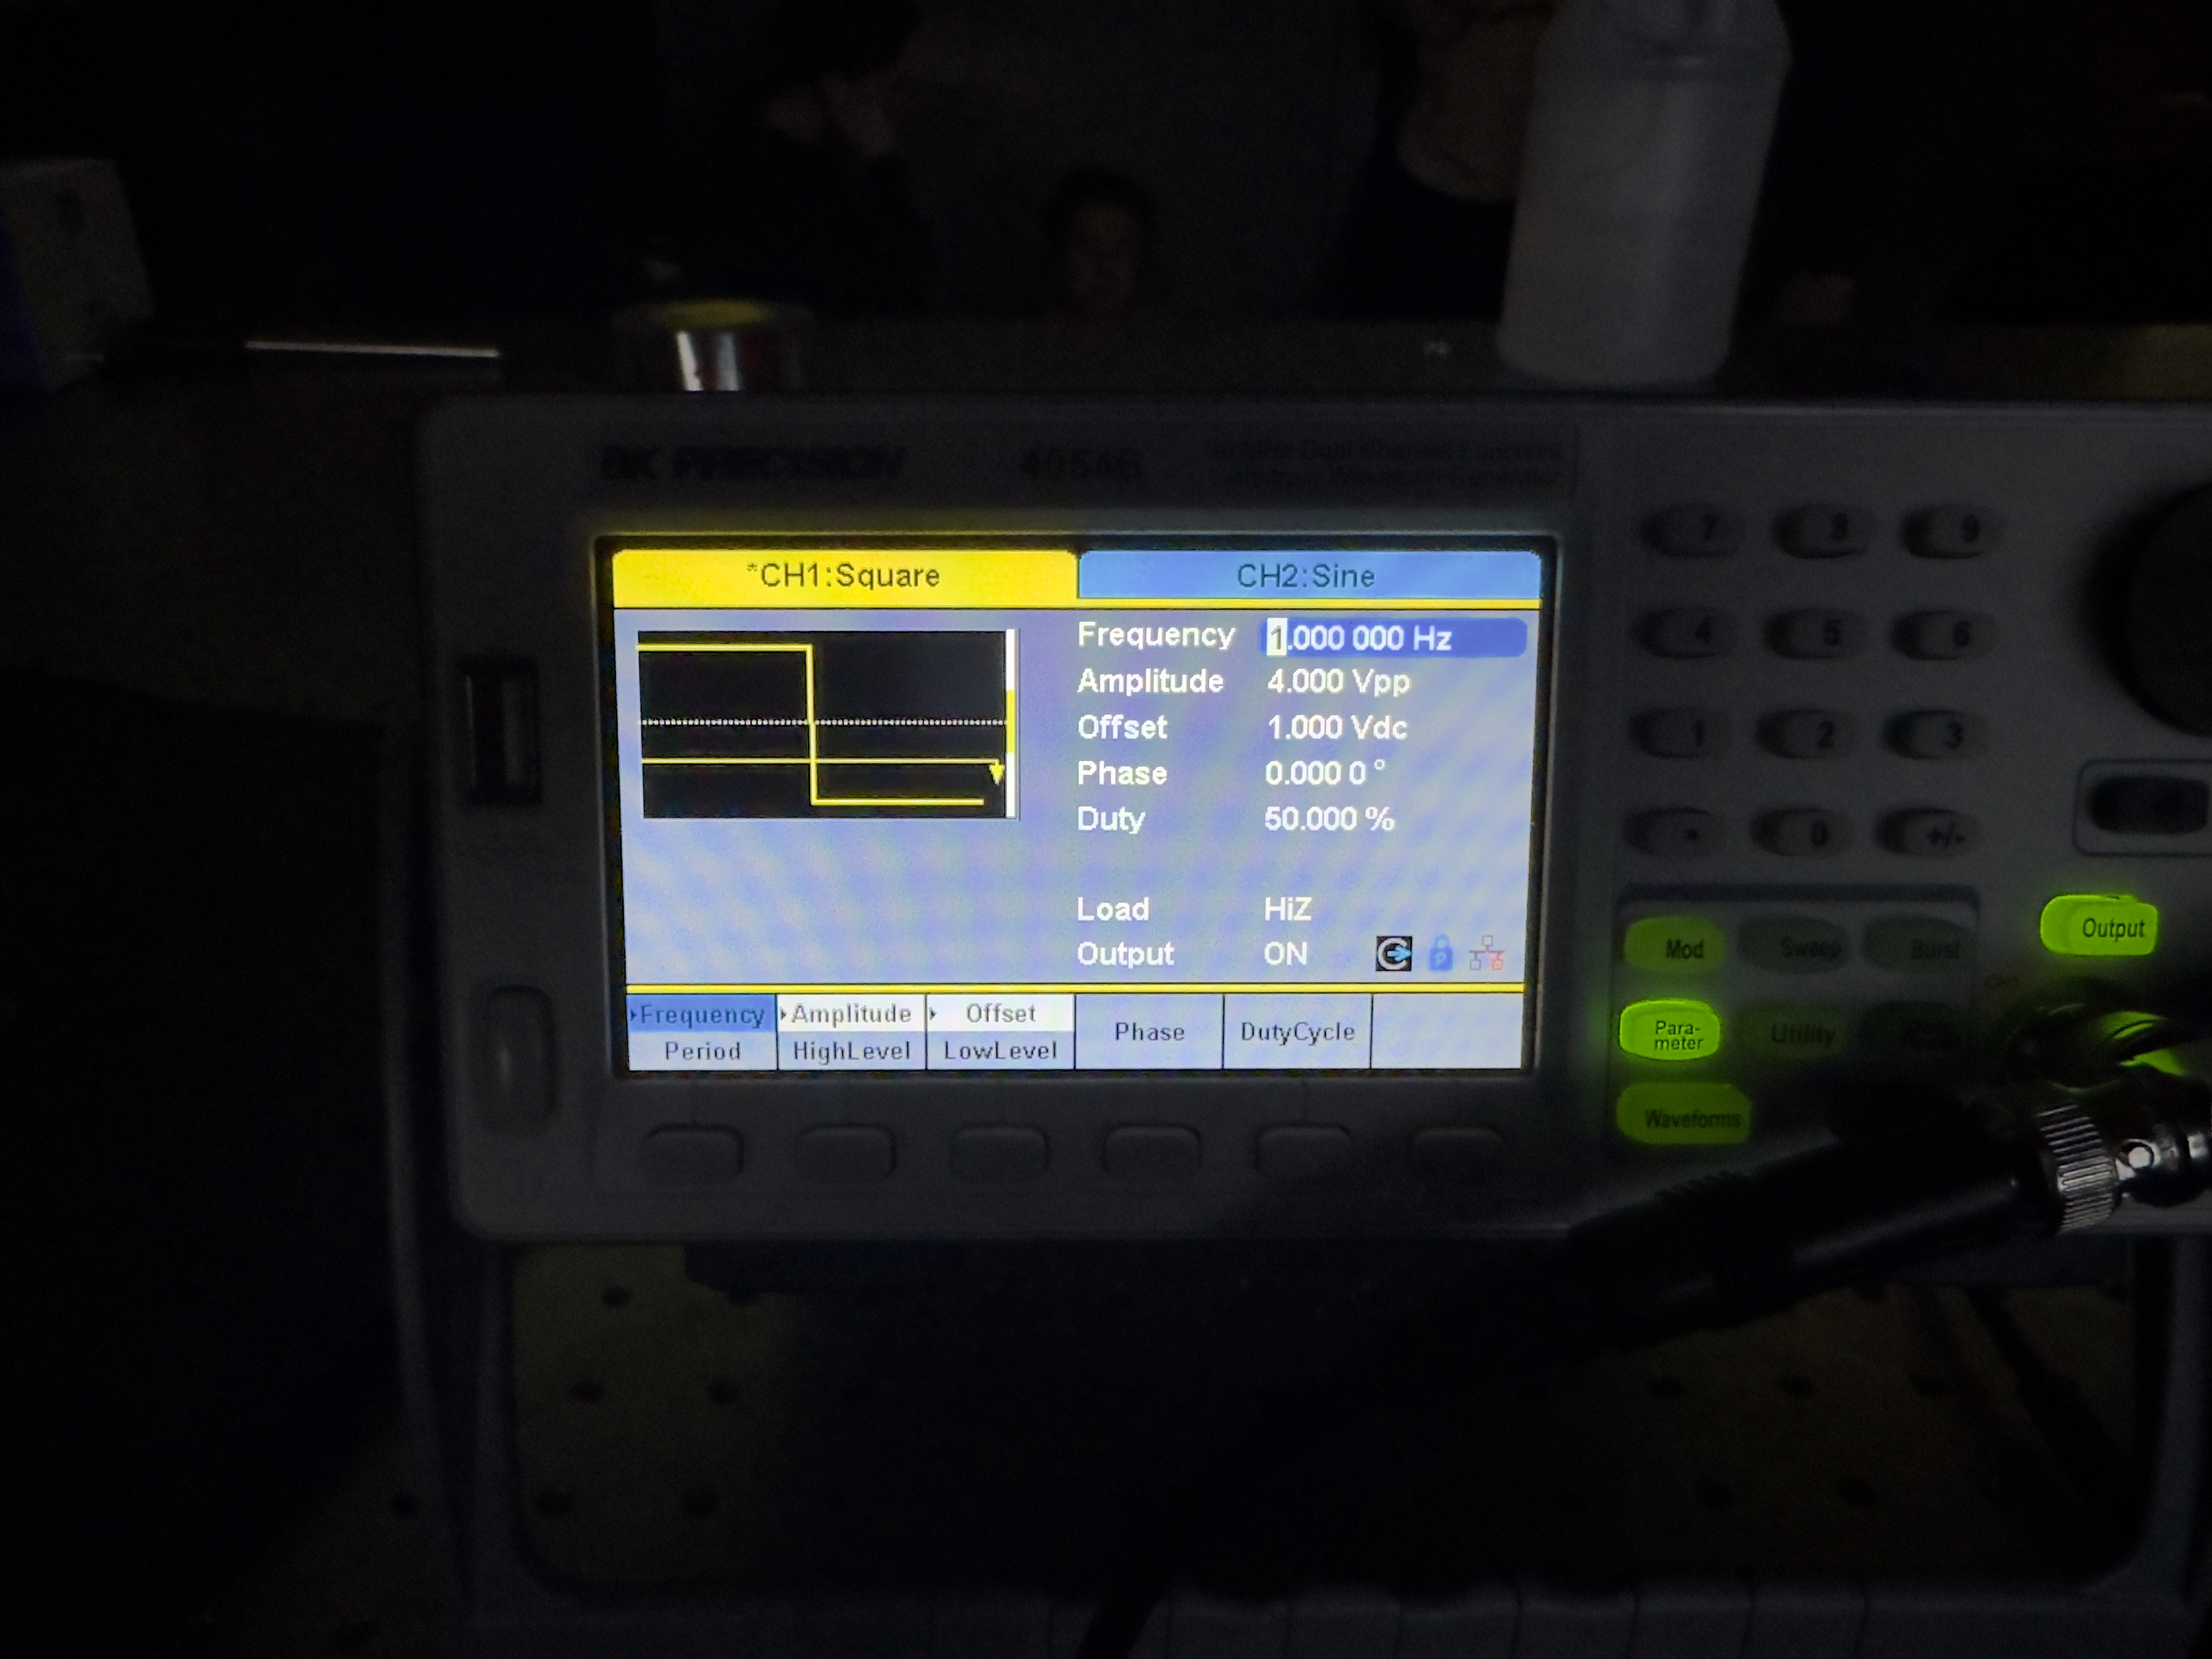
\includegraphics[width=0.75\linewidth]{Figures/delay_generator_settings.jpeg}
    \caption[Delay Generator Settings]{Delay Generator Settings}
    \label{fig: delayGeneratorsettings}
\end{figure}

\begin{figure}[htpb]
    \centering
    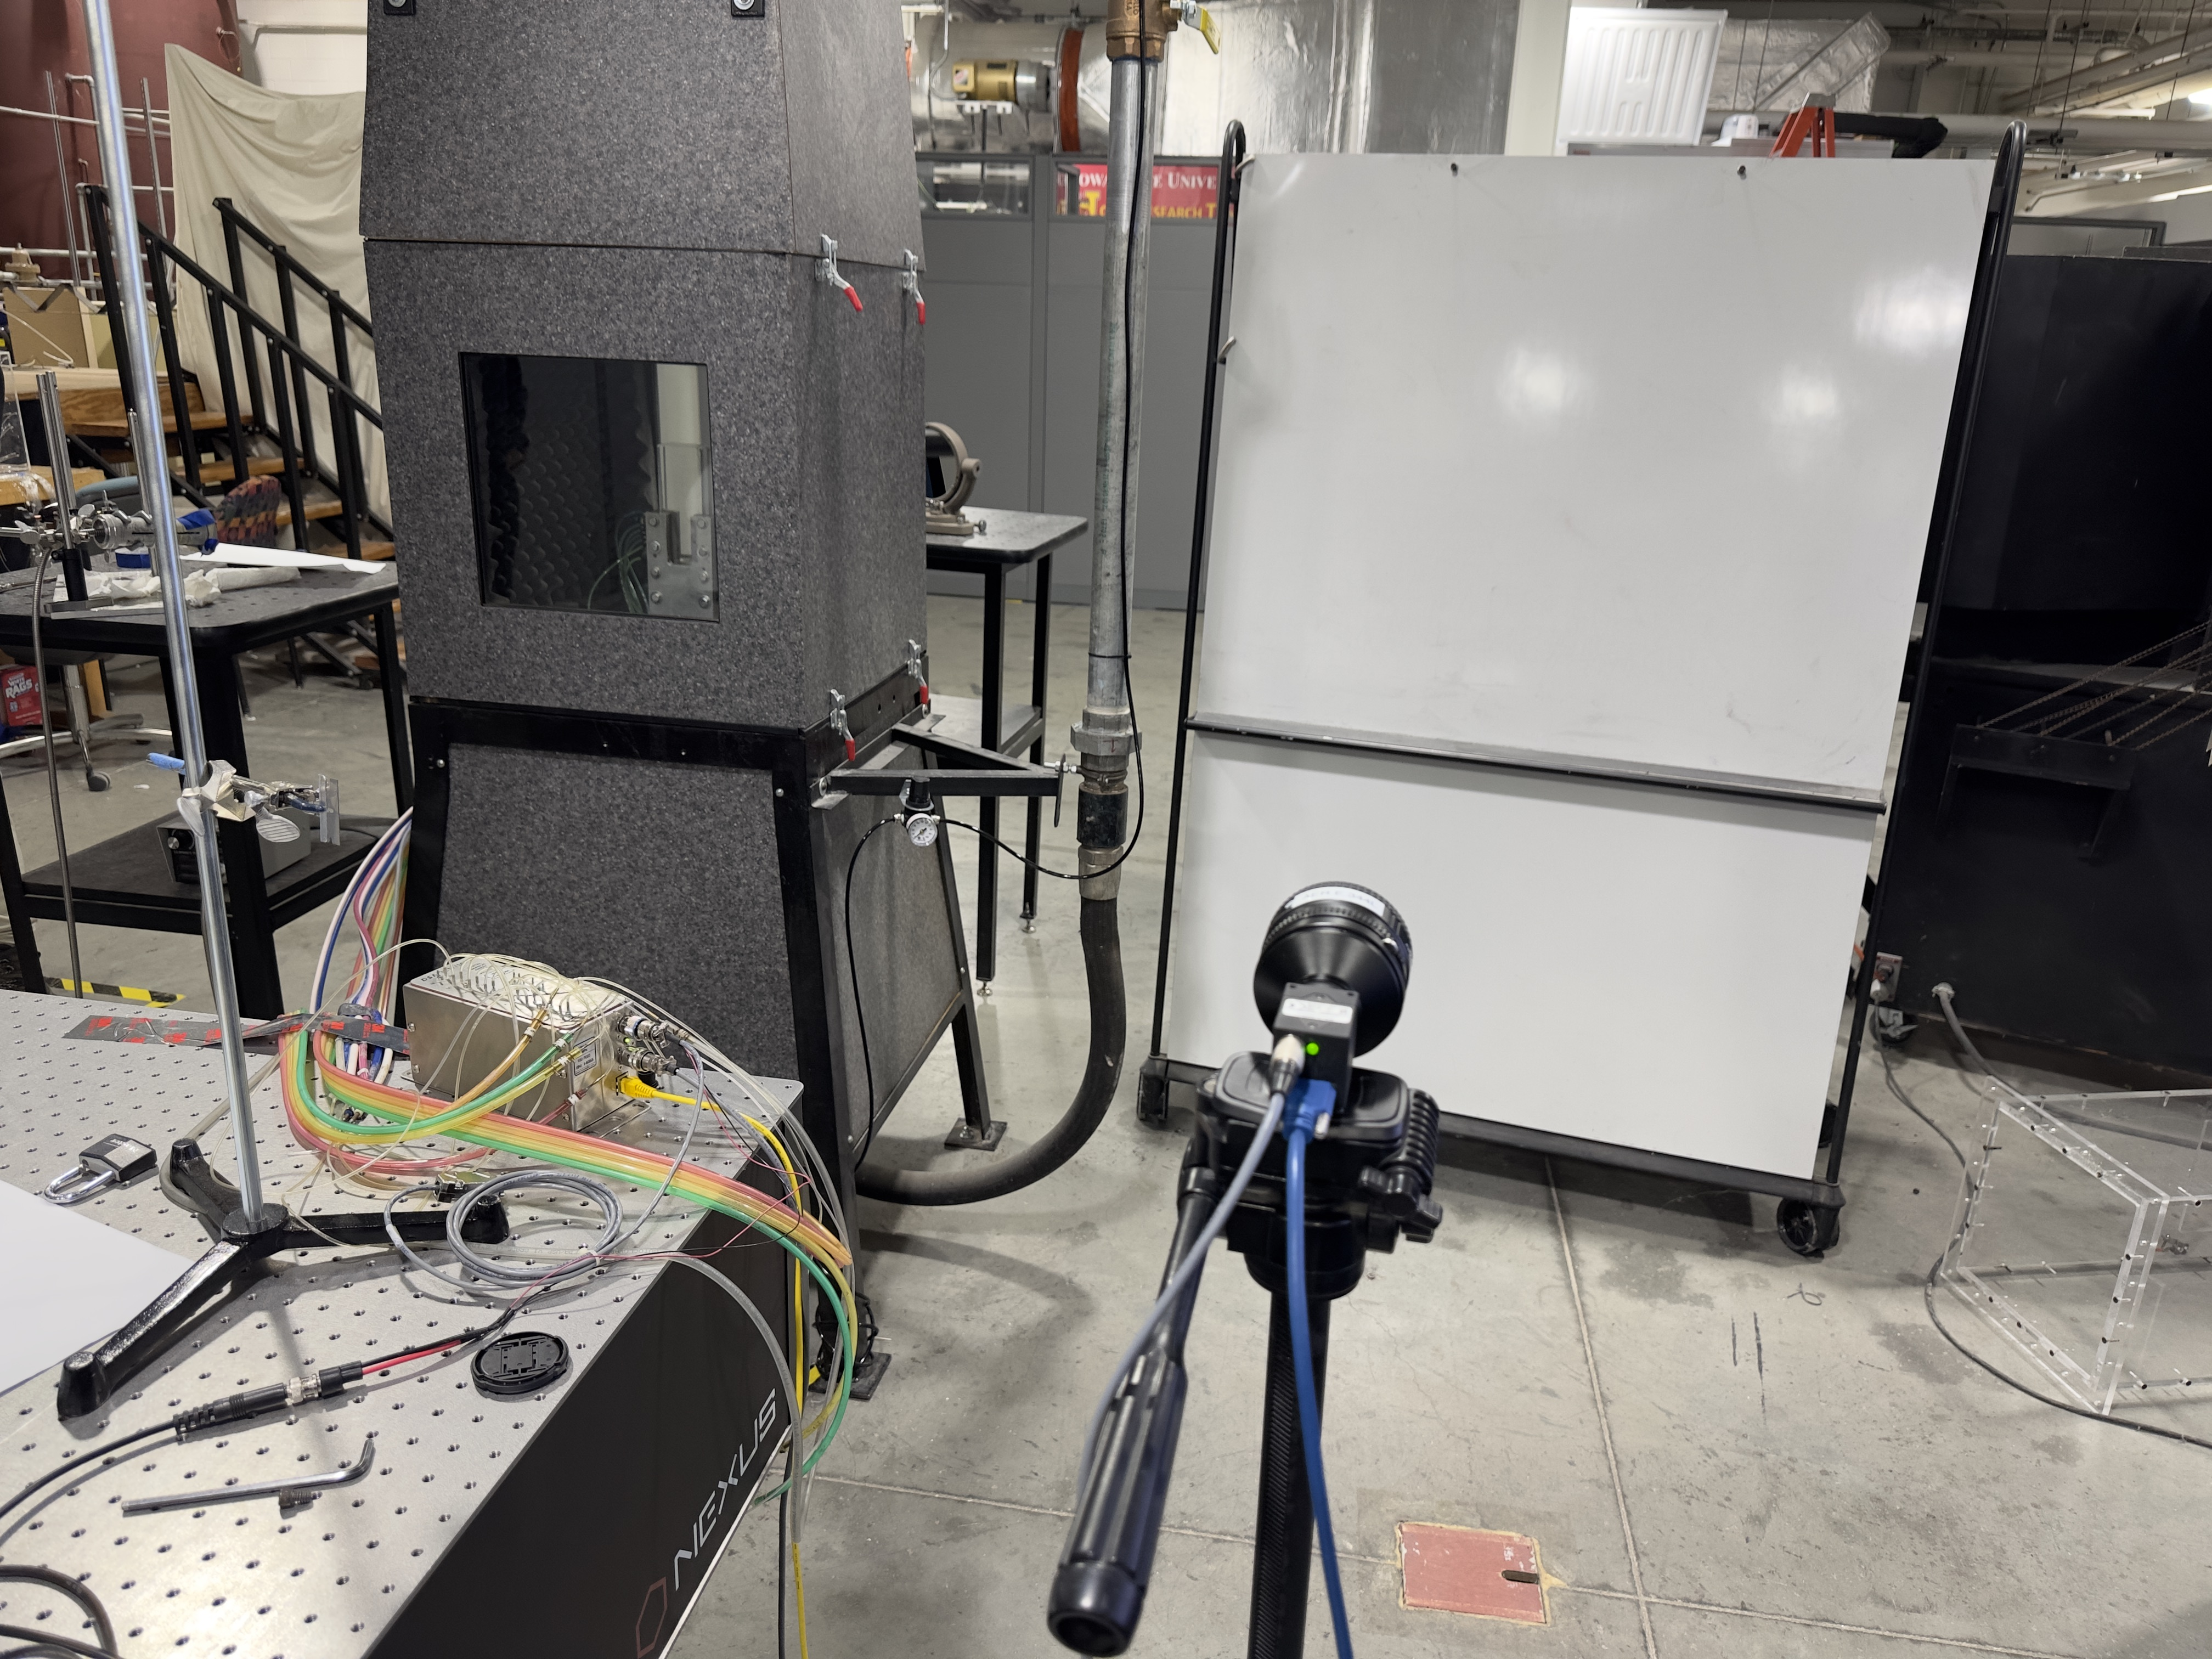
\includegraphics[width=0.75\linewidth]{Figures/schlieren_and_camera_setup.jpeg}
    \caption[schlieren and camera setup]{schlieren and camera setup}
    \label{fig: SchlierenAndCameraSetup}
\end{figure}

\begin{figure}[htpb]
    \centering
    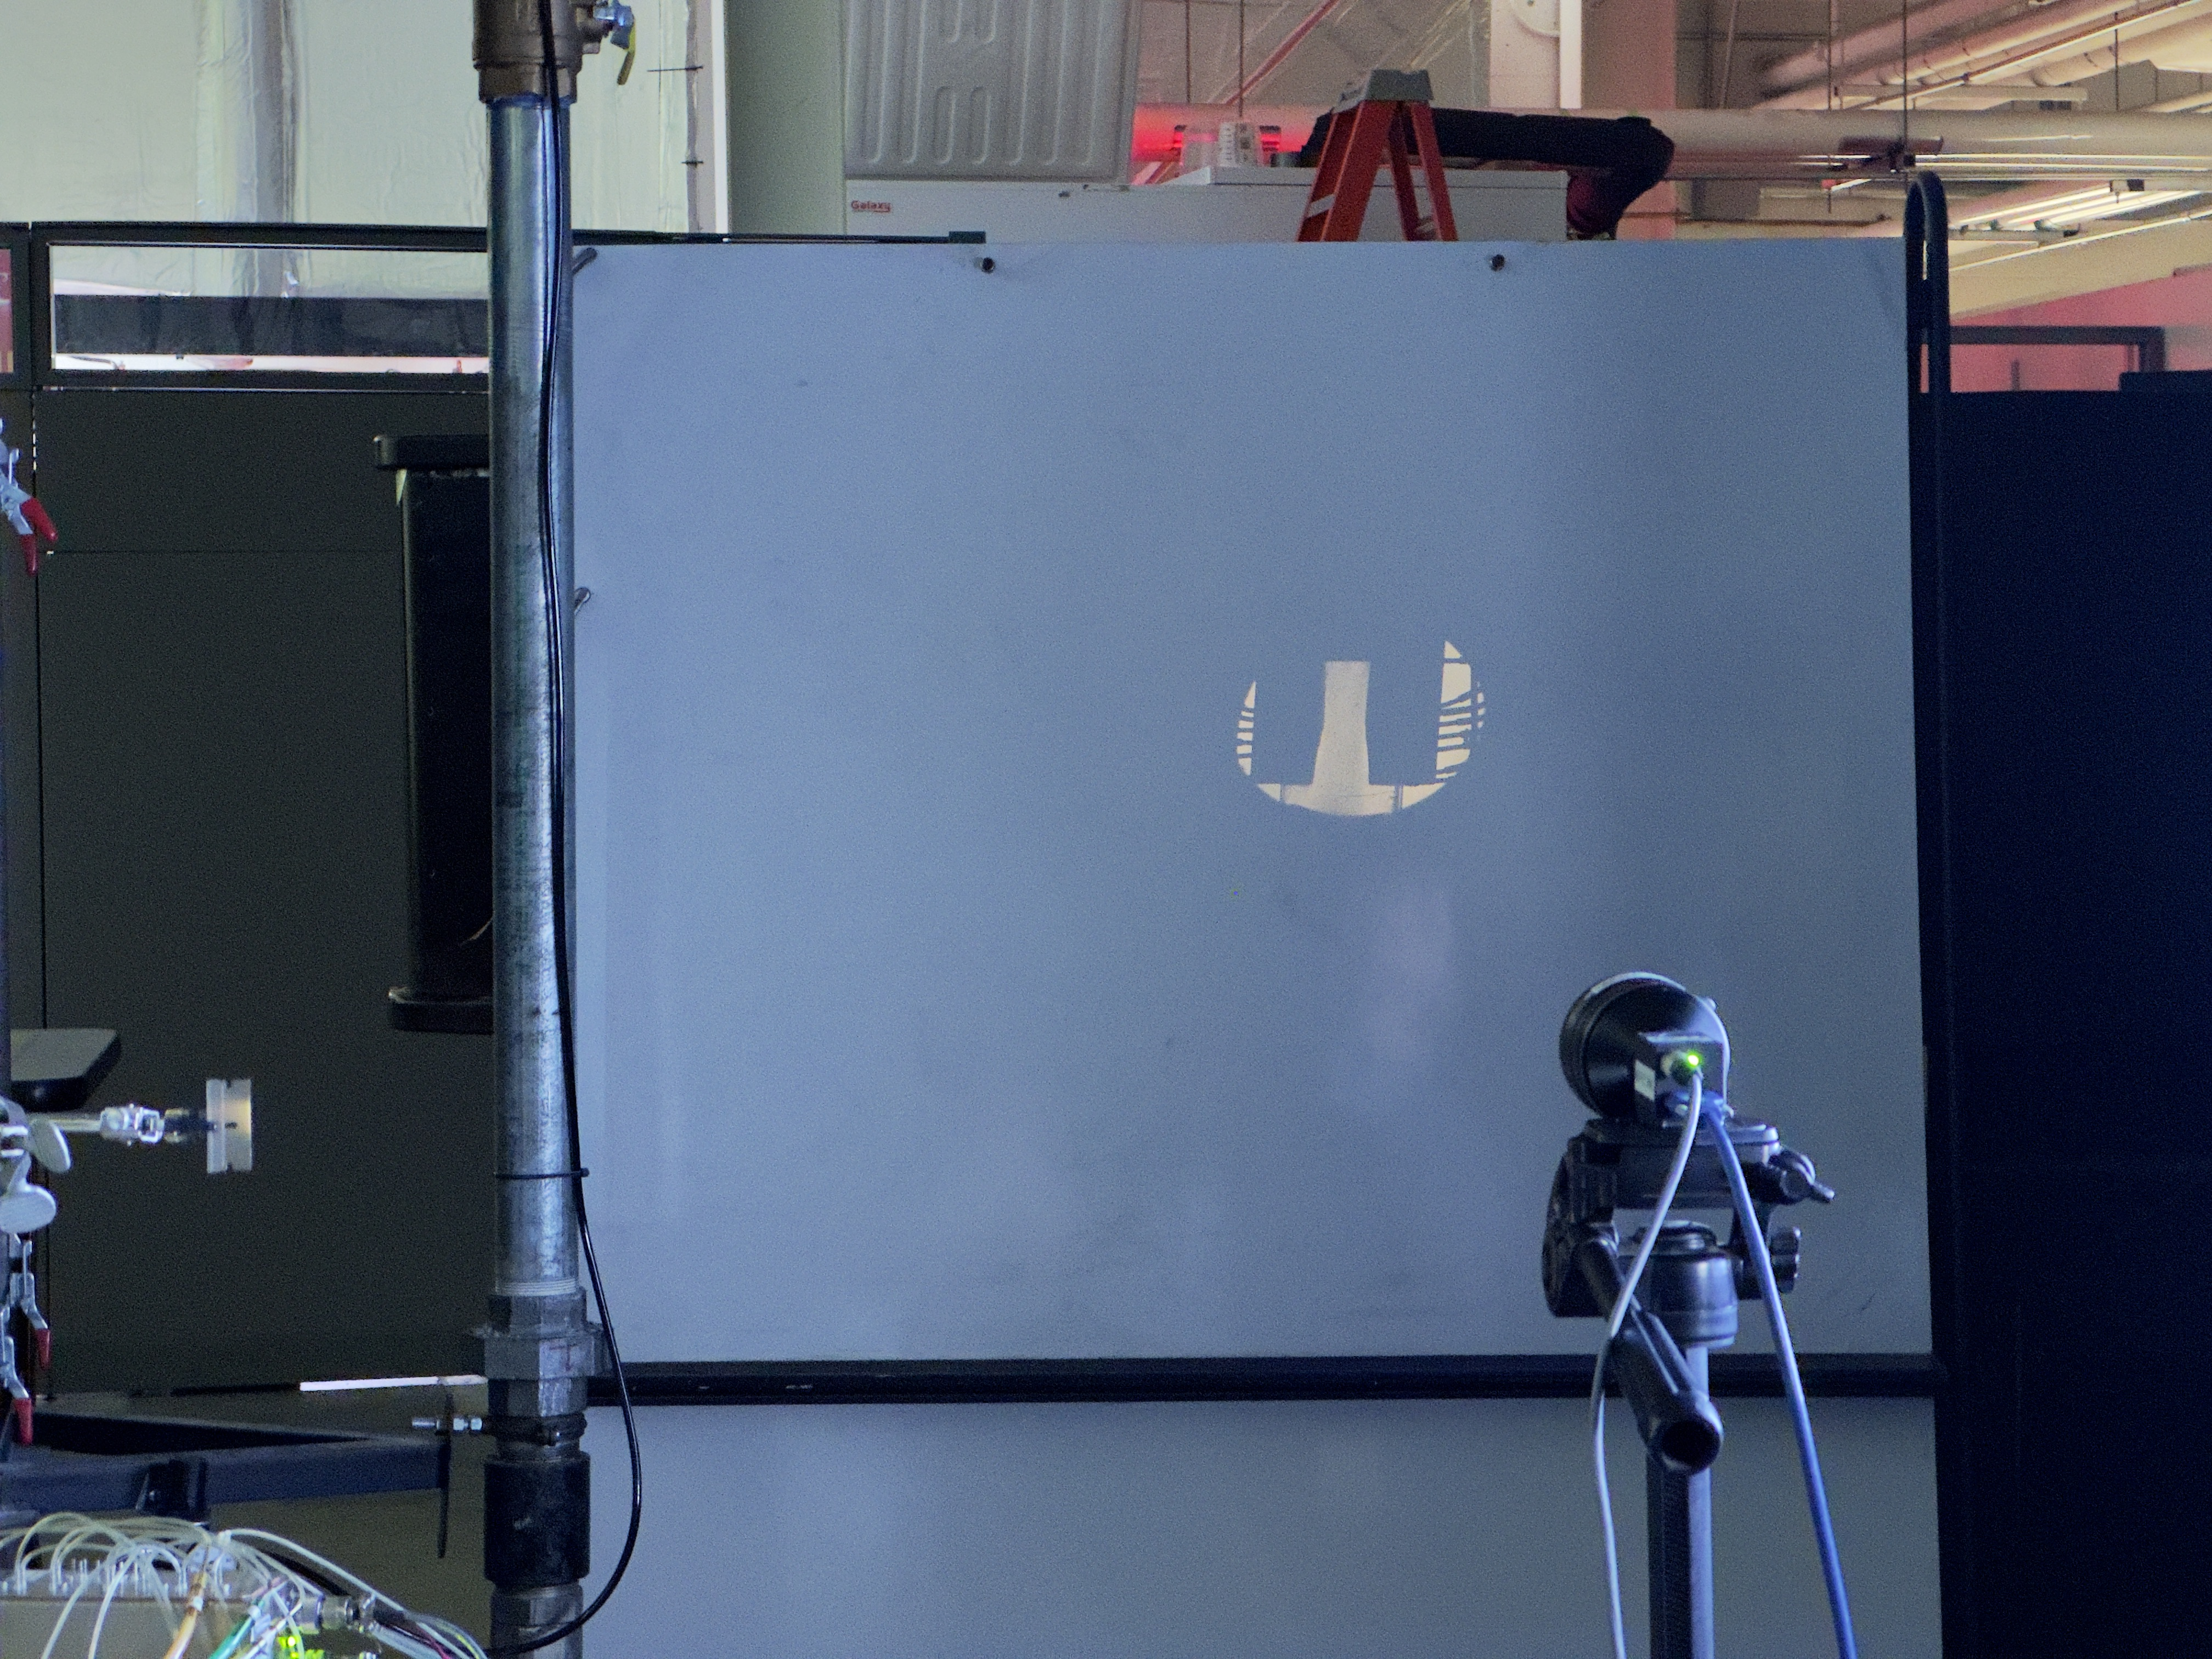
\includegraphics[width=0.75\linewidth]{Figures/schlieren_nozzle.jpeg}
    \caption[Schlieren Nozzle]{Schlieren Nozzle}
    \label{fig: SchlierenNozzle}
\end{figure}

\begin{figure}[htpb]
    \centering
    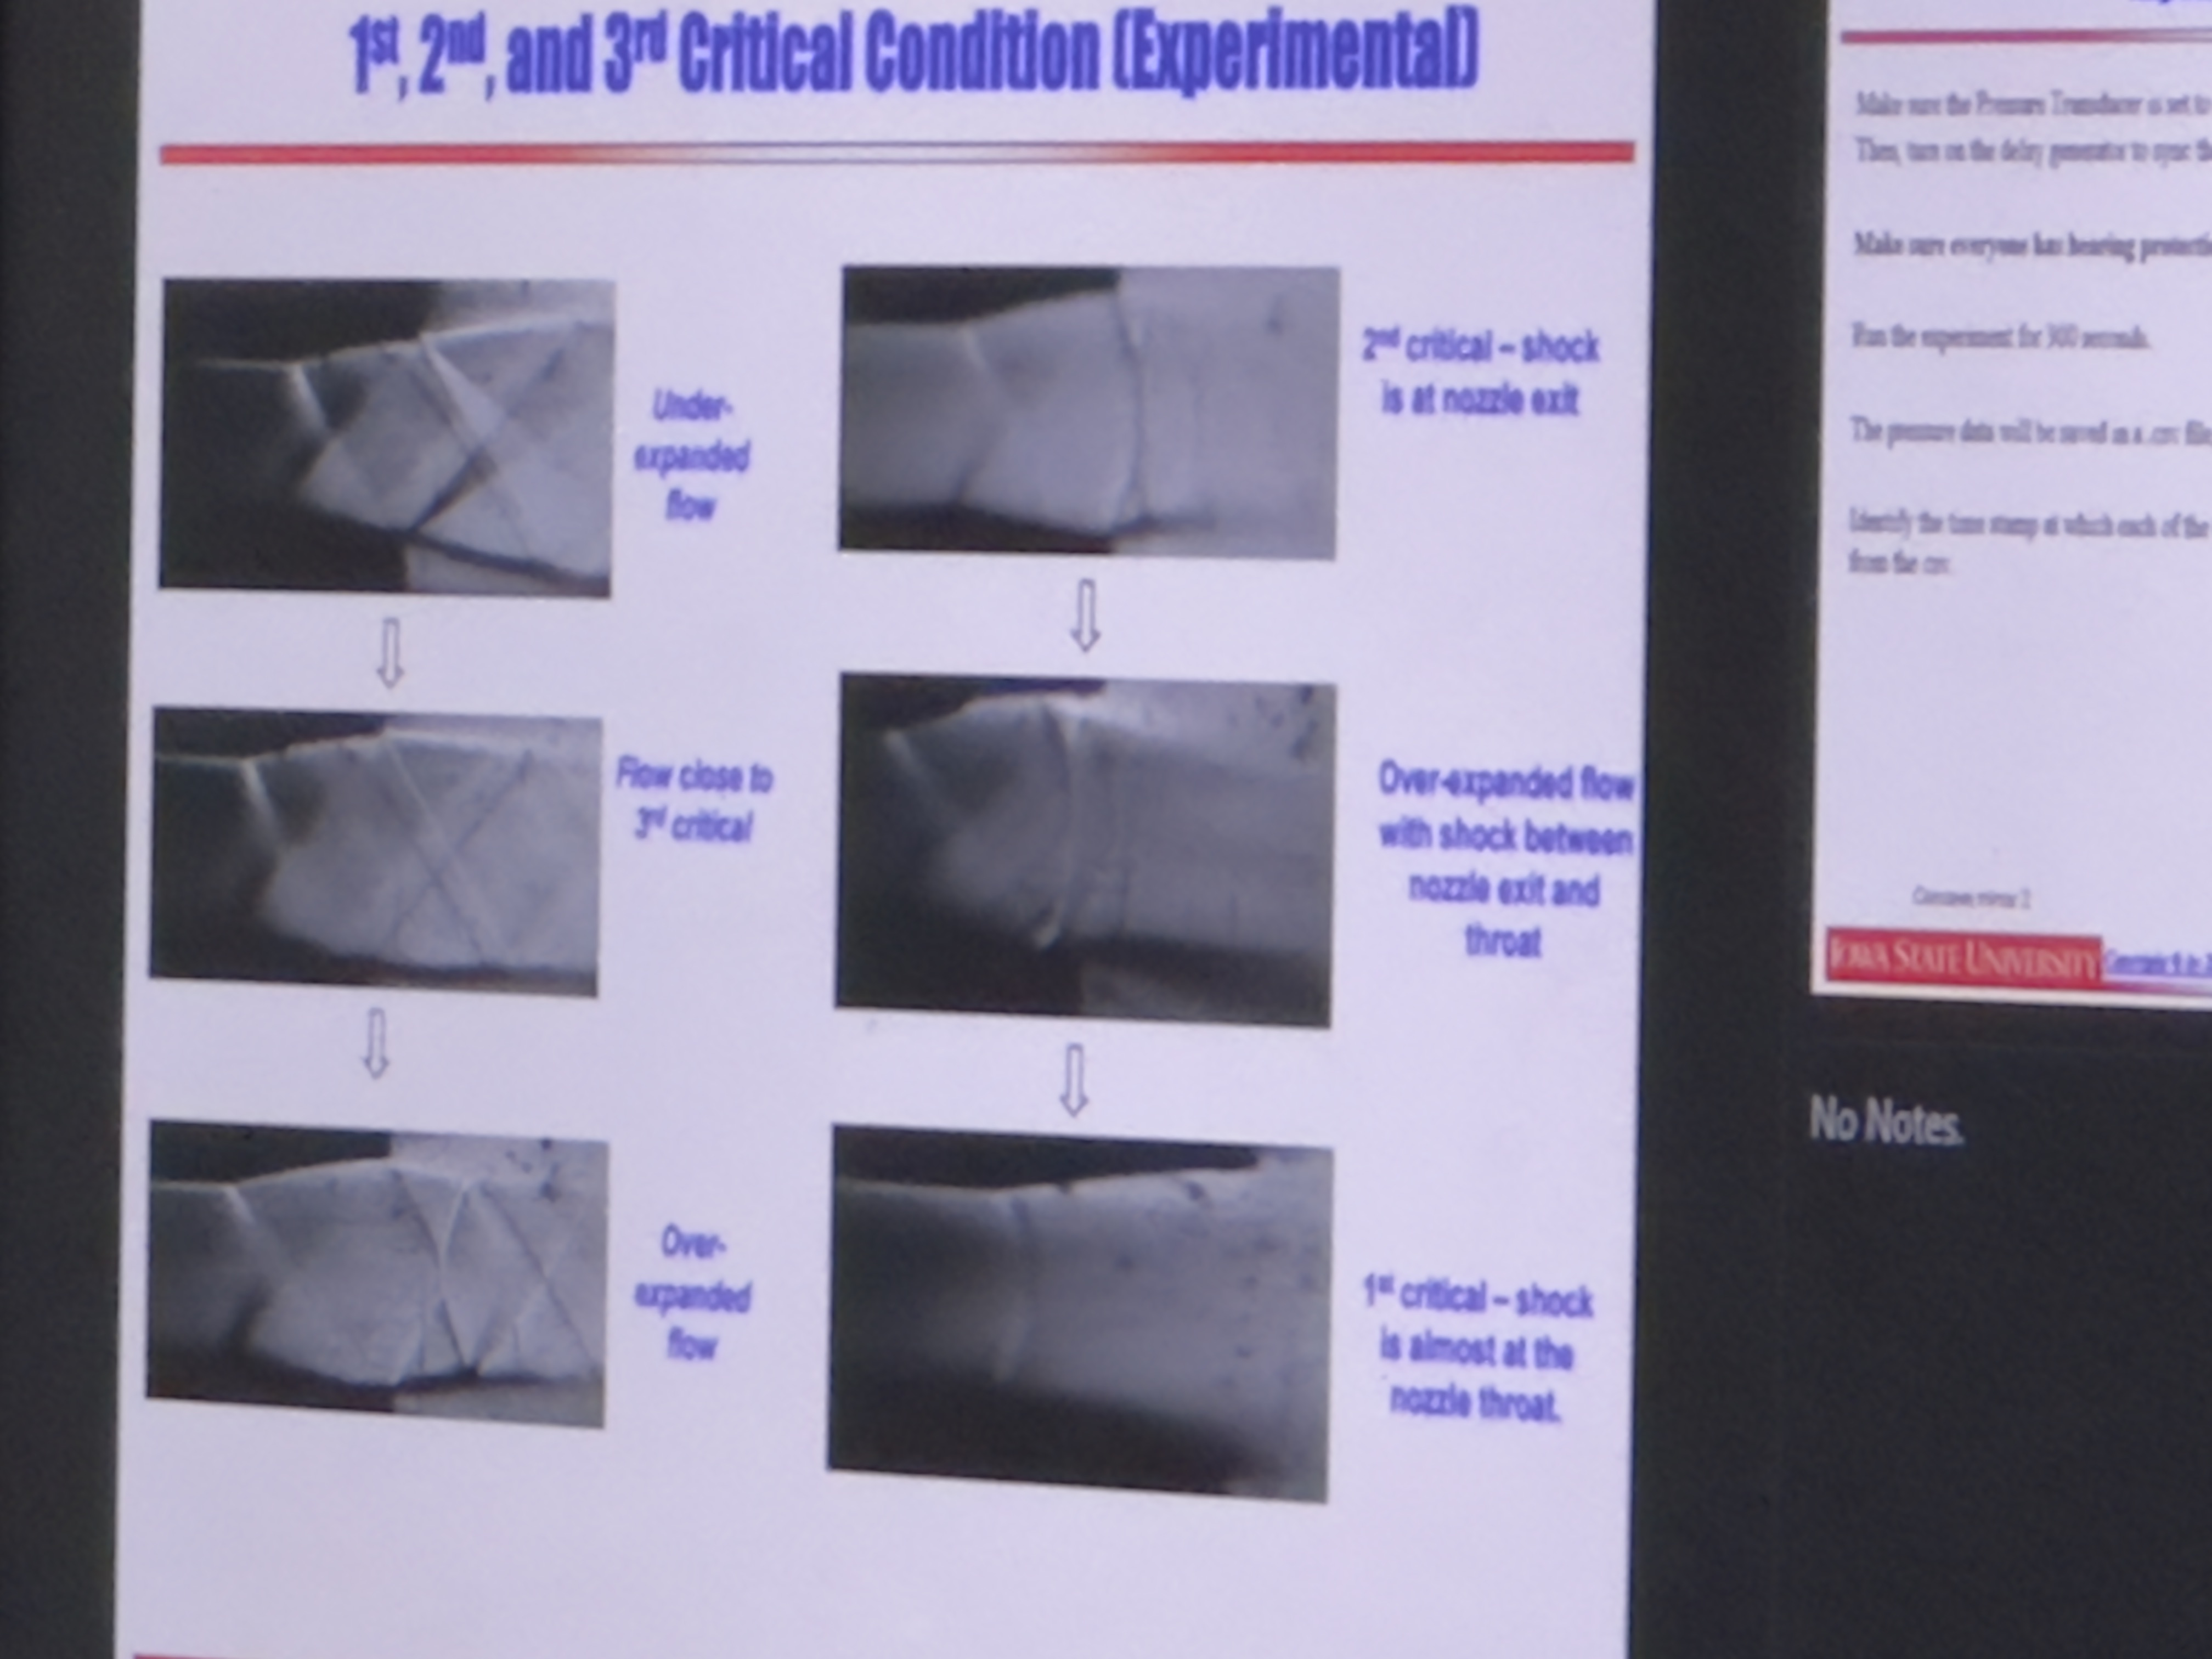
\includegraphics[width=0.75\linewidth]{Figures/six_conditions.jpeg}
    \caption[Nozzle Conditions]{Nozzle Conditions}
    \label{fig: NozzleConditions}
\end{figure}

\newpage

\section{Additional Figures} \label{sec:additional_apparatus}

\begin{figure}[htpb]
    \centering
     \includesvg[width=0.75\linewidth]{Figures/Measured Pressure Distribution - 1st Critical Condition.svg}
     \caption
     [Measured Pressure Distribution - 1st Critical Condition]
     {Measured Pressure Distribution - 1st Critical Condition}
     \label{fig: MeasuredPressureDistribution1stCriticalCondition}
\end{figure}

\begin{figure}[htpb]
    \centering
     \includesvg[width=0.75\linewidth]{Figures/Measured Pressure Distribution - 2nd Critical Condition.svg}
     \caption
     [Measured Pressure Distribution - 2nd Critical Condition]
     {Measured Pressure Distribution - 2nd Critical Condition}
     \label{fig: MeasuredPressureDistribution2ndCriticalCondition}
\end{figure}

\begin{figure}[htpb]
    \centering
     \includesvg[width=0.75\linewidth]{Figures/Measured Pressure Distribution - 3rd Critical Condition.svg}
     \caption
     [Measured Pressure Distribution - 3rd Critical Condition]
     {Measured Pressure Distribution - 3rd Critical Condition}
     \label{fig: MeasuredPressureDistribution3rdCriticalCondition}
\end{figure}

\begin{figure}[htpb]
    \centering
     \includesvg[width=0.75\linewidth]{Figures/Measured Pressure Distribution - Normal Shock Inside the Nozzle.svg}
     \caption
     [Measured Pressure Distribution - Normal Shock Inside the Nozzle]
     {Measured Pressure Distribution - Normal Shock Inside the Nozzle}
     \label{fig: MeasuredPressureDistributionNormalShockInsidetheNozzle}
\end{figure}

\begin{figure}[htpb]
    \centering
     \includesvg[width=0.75\linewidth]{Figures/Measured vs. Theoretical Mach Number - 1st Critical Condition.svg}
     \caption
     [Measured vs. Theoretical Mach Number - 1st Critical Condition]
     {Measured vs. Theoretical Mach Number - 1st Critical Condition}
     \label{fig: MeasuredvsTheoreticalMachNumber1stCriticalCondition}
\end{figure}

\begin{figure}[htpb]
    \centering
     \includesvg[width=0.75\linewidth]{Figures/Measured vs. Theoretical Mach Number - 2nd Critical Condition.svg}
     \caption
     [Measured vs. Theoretical Mach Number - 2nd Critical Condition]
     {Measured vs. Theoretical Mach Number - 2nd Critical Condition}
     \label{fig: MeasuredvsTheoreticalMachNumber2ndCriticalCondition}
\end{figure}

\begin{figure}[htpb]
    \centering
     \includesvg[width=0.75\linewidth]{Figures/Measured vs. Theoretical Mach Number - 3rd Critical Condition.svg}
     \caption
     [Measured vs. Theoretical Mach Number - 3rd Critical Condition]
     {Measured vs. Theoretical Mach Number - 3rd Critical Condition}
     \label{fig: MeasuredvsTheoreticalMachNumber3rdCriticalCondition}
\end{figure}

\begin{figure}[htpb]
    \centering
     \includesvg[width=0.75\linewidth]{Figures/Measured vs. Theoretical Mach Number - Normal Shock Inside the Nozzle.svg}
     \caption
     [Measured vs. Theoretical Mach Number - Normal Shock Inside the Nozzle]
     {Measured vs. Theoretical Mach Number - Normal Shock Inside the Nozzle}
     \label{fig: MeasuredvsTheoreticalMachNumberNormalShockInsidetheNozzle}
\end{figure}

\begin{figure}[htpb]
    \centering
     \includesvg[width=0.75\linewidth]{Figures/Measured vs. Theoretical Pressure Distribution - 1st Critical Condition.svg}
     \caption
     [Measured vs. Theoretical Pressure Distribution - 1st Critical Condition]
     {Measured vs. Theoretical Pressure Distribution - 1st Critical Condition}
     \label{fig: MeasuredvsTheoreticalPressureDistribution1stCriticalCondition}
\end{figure}

\begin{figure}[htpb]
    \centering
     \includesvg[width=0.75\linewidth]{Figures/Measured vs. Theoretical Pressure Distribution - 2nd Critical Condition.svg}
     \caption
     [Measured vs. Theoretical Pressure Distribution - 2nd Critical Condition]
     {Measured vs. Theoretical Pressure Distribution - 2nd Critical Condition}
     \label{fig: MeasuredvsTheoreticalPressureDistribution2ndCriticalCondition}
\end{figure}

\begin{figure}[htpb]
    \centering
     \includesvg[width=0.75\linewidth]{Figures/Measured vs. Theoretical Pressure Distribution - 3rd Critical Condition.svg}
     \caption
     [Measured vs. Theoretical Pressure Distribution - 3rd Critical Condition]
     {Measured vs. Theoretical Pressure Distribution - 3rd Critical Condition}
     \label{fig: MeasuredvsTheoreticalPressureDistribution3rdCriticalCondition}
\end{figure}

\begin{figure}[htpb]
    \centering
     \includesvg[width=0.75\linewidth]{Figures/Measured vs. Theoretical Pressure Distribution - Normal Shock Inside the Nozzle.svg}
     \caption
     [Measured vs. Theoretical Pressure Distribution - Normal Shock Inside the Nozzle]
     {Measured vs. Theoretical Pressure Distribution - Normal Shock Inside the Nozzle}
     \label{fig: MeasuredvsTheoreticalPressureDistributionNormalShockInsidetheNozzle}
\end{figure}

\begin{figure}[htpb]
    \centering
     \includesvg[width=0.75\linewidth]{Figures/Theoretical Pressure Distribution - 1st Critical Condition.svg}
     \caption
     [Theoretical Pressure Distribution - 1st Critical Condition]
     {Theoretical Pressure Distribution - 1st Critical Condition}
     \label{fig: TheoreticalPressureDistribution1stCriticalCondition}
\end{figure}

\begin{figure}[htpb]
    \centering
     \includesvg[width=0.75\linewidth]{Figures/Theoretical Pressure Distribution - 2nd Critical Condition.svg}
     \caption
     [Theoretical Pressure Distribution - 2nd Critical Condition]
     {Theoretical Pressure Distribution - 2nd Critical Condition}
     \label{fig: TheoreticalPressureDistribution2ndCriticalCondition}
\end{figure}

\begin{figure}[htpb]
    \centering
     \includesvg[width=0.75\linewidth]{Figures/Theoretical Pressure Distribution - 3rd Critical Condition.svg}
     \caption
     [Theoretical Pressure Distribution - 3rd Critical Condition]
     {Theoretical Pressure Distribution - 3rd Critical Condition}
     \label{fig: TheoreticalPressureDistribution3rdCriticalCondition}
\end{figure}

\begin{figure}[htpb]
    \centering
     \includesvg[width=0.75\linewidth]{Figures/Theoretical Pressure Distribution - Normal Shock Inside the Nozzle.svg}
     \caption
     [Theoretical Pressure Distribution - Normal Shock Inside the Nozzle]
     {Theoretical Pressure Distribution - Normal Shock Inside the Nozzle}
     \label{fig: TheoreticalPressureDistributionNormalShockInsidetheNozzle}
\end{figure}

